% LaTeX-Vorlage Version 3.1,  Juli 2011

 
\documentclass[a4paper,bibtotoc,oneside]{scrbook} 
% F"ur kurze Arbeiten w"are auch die Dokumentklasse "scrartcl" ausreichend. In diesem Fall ist "section" die h"ochste Ebene ("chapter" gibt es dann nicht).
% \documentclass[a4paper,bibtotoc,oneside]{scrartcl}


% verlinkte Querverweise im pdf
\usepackage{hyperref}

% deutsche Anpassungen
%\usepackage[ansinew]{inputenc}
\usepackage[utf8]{inputenc}
\usepackage[T1]{fontenc}
\usepackage[ngerman]{babel}




% mathematische Symbole
\usepackage{amsmath,amssymb,amsfonts,amstext}

% Kopfzeilen frei gestaltbar
\usepackage{fancyhdr}
\lfoot[\fancyplain{}{}]{\fancyplain{}{}}
\rfoot[\fancyplain{}{}]{\fancyplain{}{}}
\cfoot[\fancyplain{}{\footnotesize\thepage}]{\fancyplain{}{\footnotesize\thepage}}
\lhead[\fancyplain{}{\footnotesize\nouppercase\leftmark}]{\fancyplain{}{}}
\chead{}
\rhead[\fancyplain{}{}]{\fancyplain{}{\footnotesize\nouppercase\sc\leftmark}} 

% Farben im Dokument m"oglich
\usepackage{color}

% Schriftart Helvetica
\usepackage{helvet}
\renewcommand{\familydefault}{cmss} 

% Graphiken einbinden: hier f"ur pdflatex
\usepackage[pdftex]{graphicx}

\usepackage{array}

\usepackage{subfigure} 

\usepackage{multirow}

% H"ohe und Breite des Textk"orpers etwas gr"osser definieren
\setlength{\textheight}{225mm}
\setlength{\textwidth}{1.05\textwidth}

% weniger Warnungen wegen "uberf"ullter Boxen
\tolerance = 9999
\sloppy

% Anpassung einiger "Uberschriften 
\renewcommand\figurename{Abbildung}
\renewcommand\tablename{Tabelle}



\begin{document}

% Kopf- und Fusszeilen initiieren
\pagestyle{fancy}

% Deckblatt:
\thispagestyle{empty}
\begin{picture}(0,0)
\color{white}\sffamily
\put(-101,-749){
\includegraphics[width=1.002\paperwidth, height=\paperheight]{img/BM_2011.pdf}}
\put(220,-670){
\includegraphics[width=0.5\textwidth]{img/FHTW_Logo_4c.pdf}}
\put(-30, -20){\bfseries\huge MASTER THESIS}
\put(-30,-50){\Large zur Erlangung des akademischen Grades}
\put(-30,-70){\Large \glqq Master of Science in Engineering\grqq}
% Titel des Studienganges einf"ugen:
\put(-30,-90){\Large im Studiengang Industrielle Elektronik}
% Titel der Arbeit einf"ugen:
% Die Minipage wird gesetzt, damit auch mehrzeilige Titel m"oglich werden.
\put(-32,-180){
\begin{minipage}{14cm}
\bfseries\huge Aufbau eines automatisierten Mess- und Auswertesystems zur Bestimmung der Bestrahlungsst"arkeverteilung in einem station"aren Sonnensimulator
\end{minipage}
}
% Name der Autorin/des Autors eingeben:
\put(-30,-270){\large Ausgef"uhrt von: Thomas Schmatz BSc}
% Personenkennzeichen der Autorin/des Autors eingeben:
\put(-30,-290){\large Personenkennzeichen: 1010300002}
% Name der Begutachterinnen/der Begutachter eingeben:
\put(-30,-330){\large 1. BegutachterIn: DI Bernhard Kubicek}
\put(-30,-350){\large 2. BegutachterIn: DI (FH) Thomas Krametz }
\put(-30,-390){\large Wien, \today} % das Datum des letzten Kompilierens wird automatisch eingesetzt
\color{black}
\end{picture}

\newpage


\section*{Eidesstattliche Erkl"arung}\thispagestyle{empty}
\glqq Ich erkl"are hiermit an Eides statt, dass ich die vorliegende Arbeit selbst"andig angefertigt habe. 
Die aus fremden Quellen direkt oder indirekt "ubernommenen Gedanken sind als solche kenntlich gemacht. 
Die Arbeit wurde bisher weder in gleicher noch in "ahnlicher Form einer anderen Prüfungsbehörde vorgelegt
und auch noch nicht ver"offentlicht. Ich versichere, dass die abgegebene Version jener im Uploadtool entspricht.\grqq\\[5\baselineskip]
\rule{5cm}{0.2pt}\hfill\rule{5cm}{0.2pt}\\
\phantom{Datum }Ort, Datum\hfill Unterschrift\hspace{15mm}

\newpage



\section*{Kurzfassung}\thispagestyle{empty}
Die Arbeit umfasst die Planung und Realisierung eines selbstfahrenden Messroboters, der die Bestrahlungsst"arkeverteilung in der Prüfebene eines station"aren Sonnensimulators erfasst. Neben den Einstrahlungsdaten werden werden zus"atzliche Informationen über die Umgebungsbedingungen im Prüfkanal aufgezeichnet. Bei der Umsetzung wurden Rapid-Prototyping Techniken (3D-Druck, Platinenfräse und Lasercutter) eingesetzt. Behandelt werden theoretische Grundlagen und normative Anforderungen an station"are Sonnensimulatoren, sowie Messunsicherheitsberechnungen und Validierung des Gesamtsystems.
\\ \vfill
% Bitte 3-5 deutsche Schlagw"orter eingeben, die die Arbeit charakterisieren:
\paragraph*{Schlagw"orter:} Sonnensimulator, Messroboter, Bestrahlungsstärke


\newpage

\section*{Abstract}\thispagestyle{empty}
This paper discripes the planning and the realisation of a autonomous measurement robot. The robot measures the irradiance in a test plane of a continous solar simulator.
\\ \vfill
% Bitte 3-5 englische Keywords eingeben, die die Arbeit charakterisieren:
\paragraph*{Keywords:} Measurement Robot, Measurment of Solar Radiation, Arduino, Mecanum Wheel, Keyword 5
\newpage

\section*{Danksagung}\thispagestyle{empty}
Ich danke meinen Eltern für die Unterstützung und Geduld, die sie während des Studiums aufgebracht haben.
Ich danke meinen Hochschulbetreuer für die umfangreiche Betreuung.
Ich danke meinen Firmenbetreuer Thomas Krametz für die Zeit die er sich genommen hat.
Und für problemlose Verlängerung meines Praktikums und der Diplomarbeit schulde ich Herrn Wolfgang Hribernik Wolfgang großen Dank.
\newpage

\tableofcontents\thispagestyle{empty}
\newpage

\setcounter{page}{1}

% Falls die Kapitel"uberschriften zu lang f"ur die Kopfzeile oder das Inhaltsverzeichnis sind, so erzielt man
% dort Kurzformen der Kapitelbezeichnungen mittels:
% \chapter[Kurzform]{Lange "Uberschrift}
\chapter{Aufgabenstellung}

Dieses Kapitel beschreibt die Notwendigkeit von Messungen im stationären Sonnensimulator, den Aufbau eines solchen Simulators, sowie dessen normativen Anforderungen. Ferner wird die Funktion einer Photovoltaik-Zelle beschrieben.

\section{Stationäre Photovoltaik Sonnensimulatoren} \thispagestyle{empty}

Photovoltaik-Sonnensimulatoren werden zur elektrischen Charakterisierung und Prüfung von Photovoltaik-Modulen verwendet. Der wesentliche Vorteil liegt darin, dass die Durchführung unter reproduzierbaren Umweltbedingungen (Bestrahlungsstärke, spektrale Zusammensetzung des einfallenden Lichtes und die Prüfgutstemperatur)  ermöglicht wird. Grundsätzlich werden bei konventionellen Systemen gepulste und stationäre Simulatoren, welche kontinuierlich leuchten, unterschieden. Erstere brauchen weniger Energie und heizen die Messobjekte nicht auf, und werden für die Leistungsmessung von Zellen und Modulen verwendet. Allerdings ist Blitzlänge bauartbedingt auf wenige Millisekunden begrenzt. Stationäre Simulatoren werden für Voralterung von Modulen verwendet.
Im Allgemeinen werden Messergebnisse auf Standard-Prüfbedingungen (STC) bezogen, die durch 1000W/m$^2$, 25$^{\circ}$C und AM1.5 definiert ist. Die Air Mass (AM) beschreibt das Verhältnis des Weges des einfallenden Sonnenlichtes durch die Atmosphäre bezogen auf senkrechten Einfall (siehe Abbildung \ref{airmass}). Je länger der Weg des Lichtes durch die Atmosphäre desto größer ist der Einfluss durch Streuung, Reflexion und Absorption, was sowohl die Stärke der Einstrahlung als auch die spektrale Zusammensetzung des Sonnenlichtes vom Sonnenstand abhängig macht. 
\begin{equation}
     AM = \frac {L} {L_0} \approx \frac{1}{cos~ z}
\end{equation}
Wobei L die Länge des Weges des Sonnenlichtes durch die Atmosphäre, L$_0$ die Weglänge bei senkrechten Einfall und z der Zenitwinkel des Sonnenstandes in Grad ist (\cite{wurf} S. 30). Dabei handelt es sich um eine Näherung, welche die Krümmung der Erdoberfläche und der Atmosphäre vernachlässigt. Für kleine Werte der Air Mass ist die Näherung aber hinreichend genau.
Die spektrale Verteilung des Referenzsonnenspektrums AM1.5 (siehe Abbildung \ref{sunspec}) ist durch die Norm IEC 60904-3 \cite{norm3} festgelegt. Das Spektrum des Sonnenlichtes im Weltall AM0 entspricht in etwa der thermische Strahlung eines schwarzen Körpers mit 5250$^\circ$C.
Die meisten am Markt erhältliche Sonnensimulatoren für Modulgröße (1,6 m$^2$) können das Spektrum nicht verändern, da sie Metallhalogenid-Lampen verwenden, sie sind also für einen Sonnenstand beschränkt. Es gibt Sonnensimulatoren auf LED-Basis. Das gewünschte Spektrum wird dort mit vielen LEDs unterschiedlicher Wellenlänge realisiert, somit sind auch unterschiedliche Spektren und Bestrahlungsstärken realisierbar. Das beschränkt sich zurzeit auf Simulatoren in Zellgröße.  Es gibt bereits LED-Sonnensimulatoren für Module am Markt. (\cite{mps}) Ein Vorteil dieses Systems ist die lange Lebensdauer der Lampen, welche für 10 Millionen Messungen reicht. 

\begin{figure}[htbp]
\centering
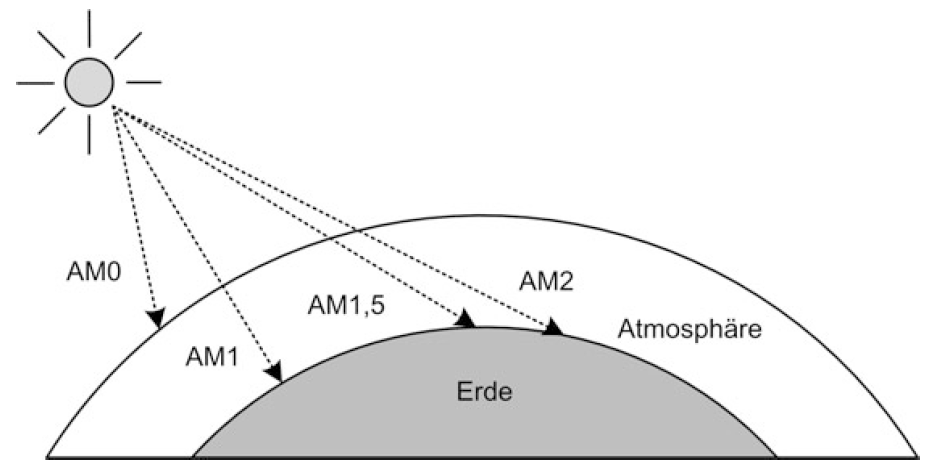
\includegraphics[width=125mm]{img/airmass2.png}
\caption[Sonnenspektrum]{Der Weg des AM0, AM1, AM1.5 und AM2-Spektrums durch die Athmosphäre. Quelle: \cite{pv}}\label{airmass}
\end{figure}

\begin{figure}[htbp]
\centering
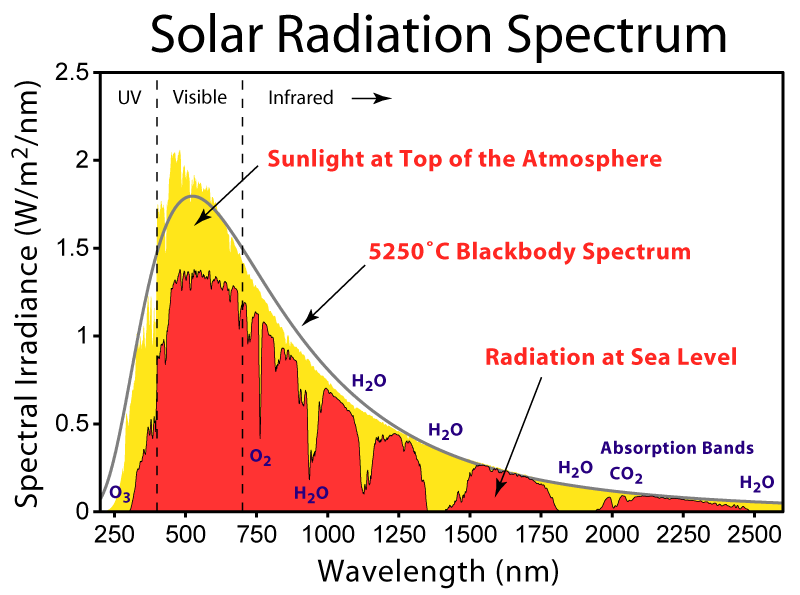
\includegraphics[width=125mm]{img/Solar_Spectrum.png}
\caption[Sonnenspektrum]{Der Vergleich von Spektrum des Sonnenlichtes im Weltall (AM0), der Strahlung eines schwarzen Körpers von 5250$^{\circ}$C und dem AM1.5 Spektrum. Quelle: \cite{sun}}\label{sunspec}
\end{figure}


\section{Sonnensimulator Aufbau}\thispagestyle{empty}


Mit der SolarConstant 4000 (siehe Abbildung \ref{sunsim}) der Firma Atlas kann die Einwirkung der Sonne auf Testobjekte simuliert werden. Dazu ist das Gerät mit zehn Metallhalogenid-Strahlungsquelle Lampen zu je 4kW. Durch die Füllung der Lampen mit Halogeniden wird ein möglichst kontinuierliches Spektrum erzeugt. Die Leuchten sind mit Filterscheiben ausgestattet, welche das abgestrahlte Licht dem AM1.5 Spektrum annähern.
Jede Lampe wird von einem eigenen elektronisch geregelten Vorschaltgerät versorgt, welches für einen gleichmäßigen und flimmerfreien Betrieb sorgt.
Da die Lampen nicht für eine Heißzündung ausgelegt sind, und dabei eventuell zerstört werden können, ist eine Sperrzeit von 10 Minuten zum Abkülen vorgesehen, bevor die Lampen wieder eingeschaltet werden können.
Die Strahlungsleistung lässt sich reduzieren indem das gesamte Lampenfeld in die Höhe gefahren wird.
Weiters lässt sich die Bestrahlungsstärke einzelner Lampen über die Variation der elektrischen Leistung des Vorschaltgerätes variieren.
Allerdings führt eine Variation der elektrischen Leistung zu einer Änderung der spektralen Strahlungsverteilung. Aus diesem Grund wird vom Hersteller empfohlen, die Helligkeit der Lampen nur zwischen 80 und 100 \% zu variieren.
Die Testobjekte werden mittels Prüfgut-Einschub in einem Windkanal positioniert, dessen obere Abdeckung aus einem geeigneten Solarglas besteht. Die geneigte Glasplatte bewirkt eine Querschnittreduktion des Luftkanales und somit eine Erhöhung der Strömungsgeschwindigkeit zwischen Zuluft- und Abluftseite. Diese stetige Erhöhung der Geschwindigkeit ist notwendig, damit die sich erwärmende Zuluft eine konstante Kühlwirkung hat, um die Testobjekt auf konstanter Temperatur zu halten.


\begin{figure}[htbp]
\centering
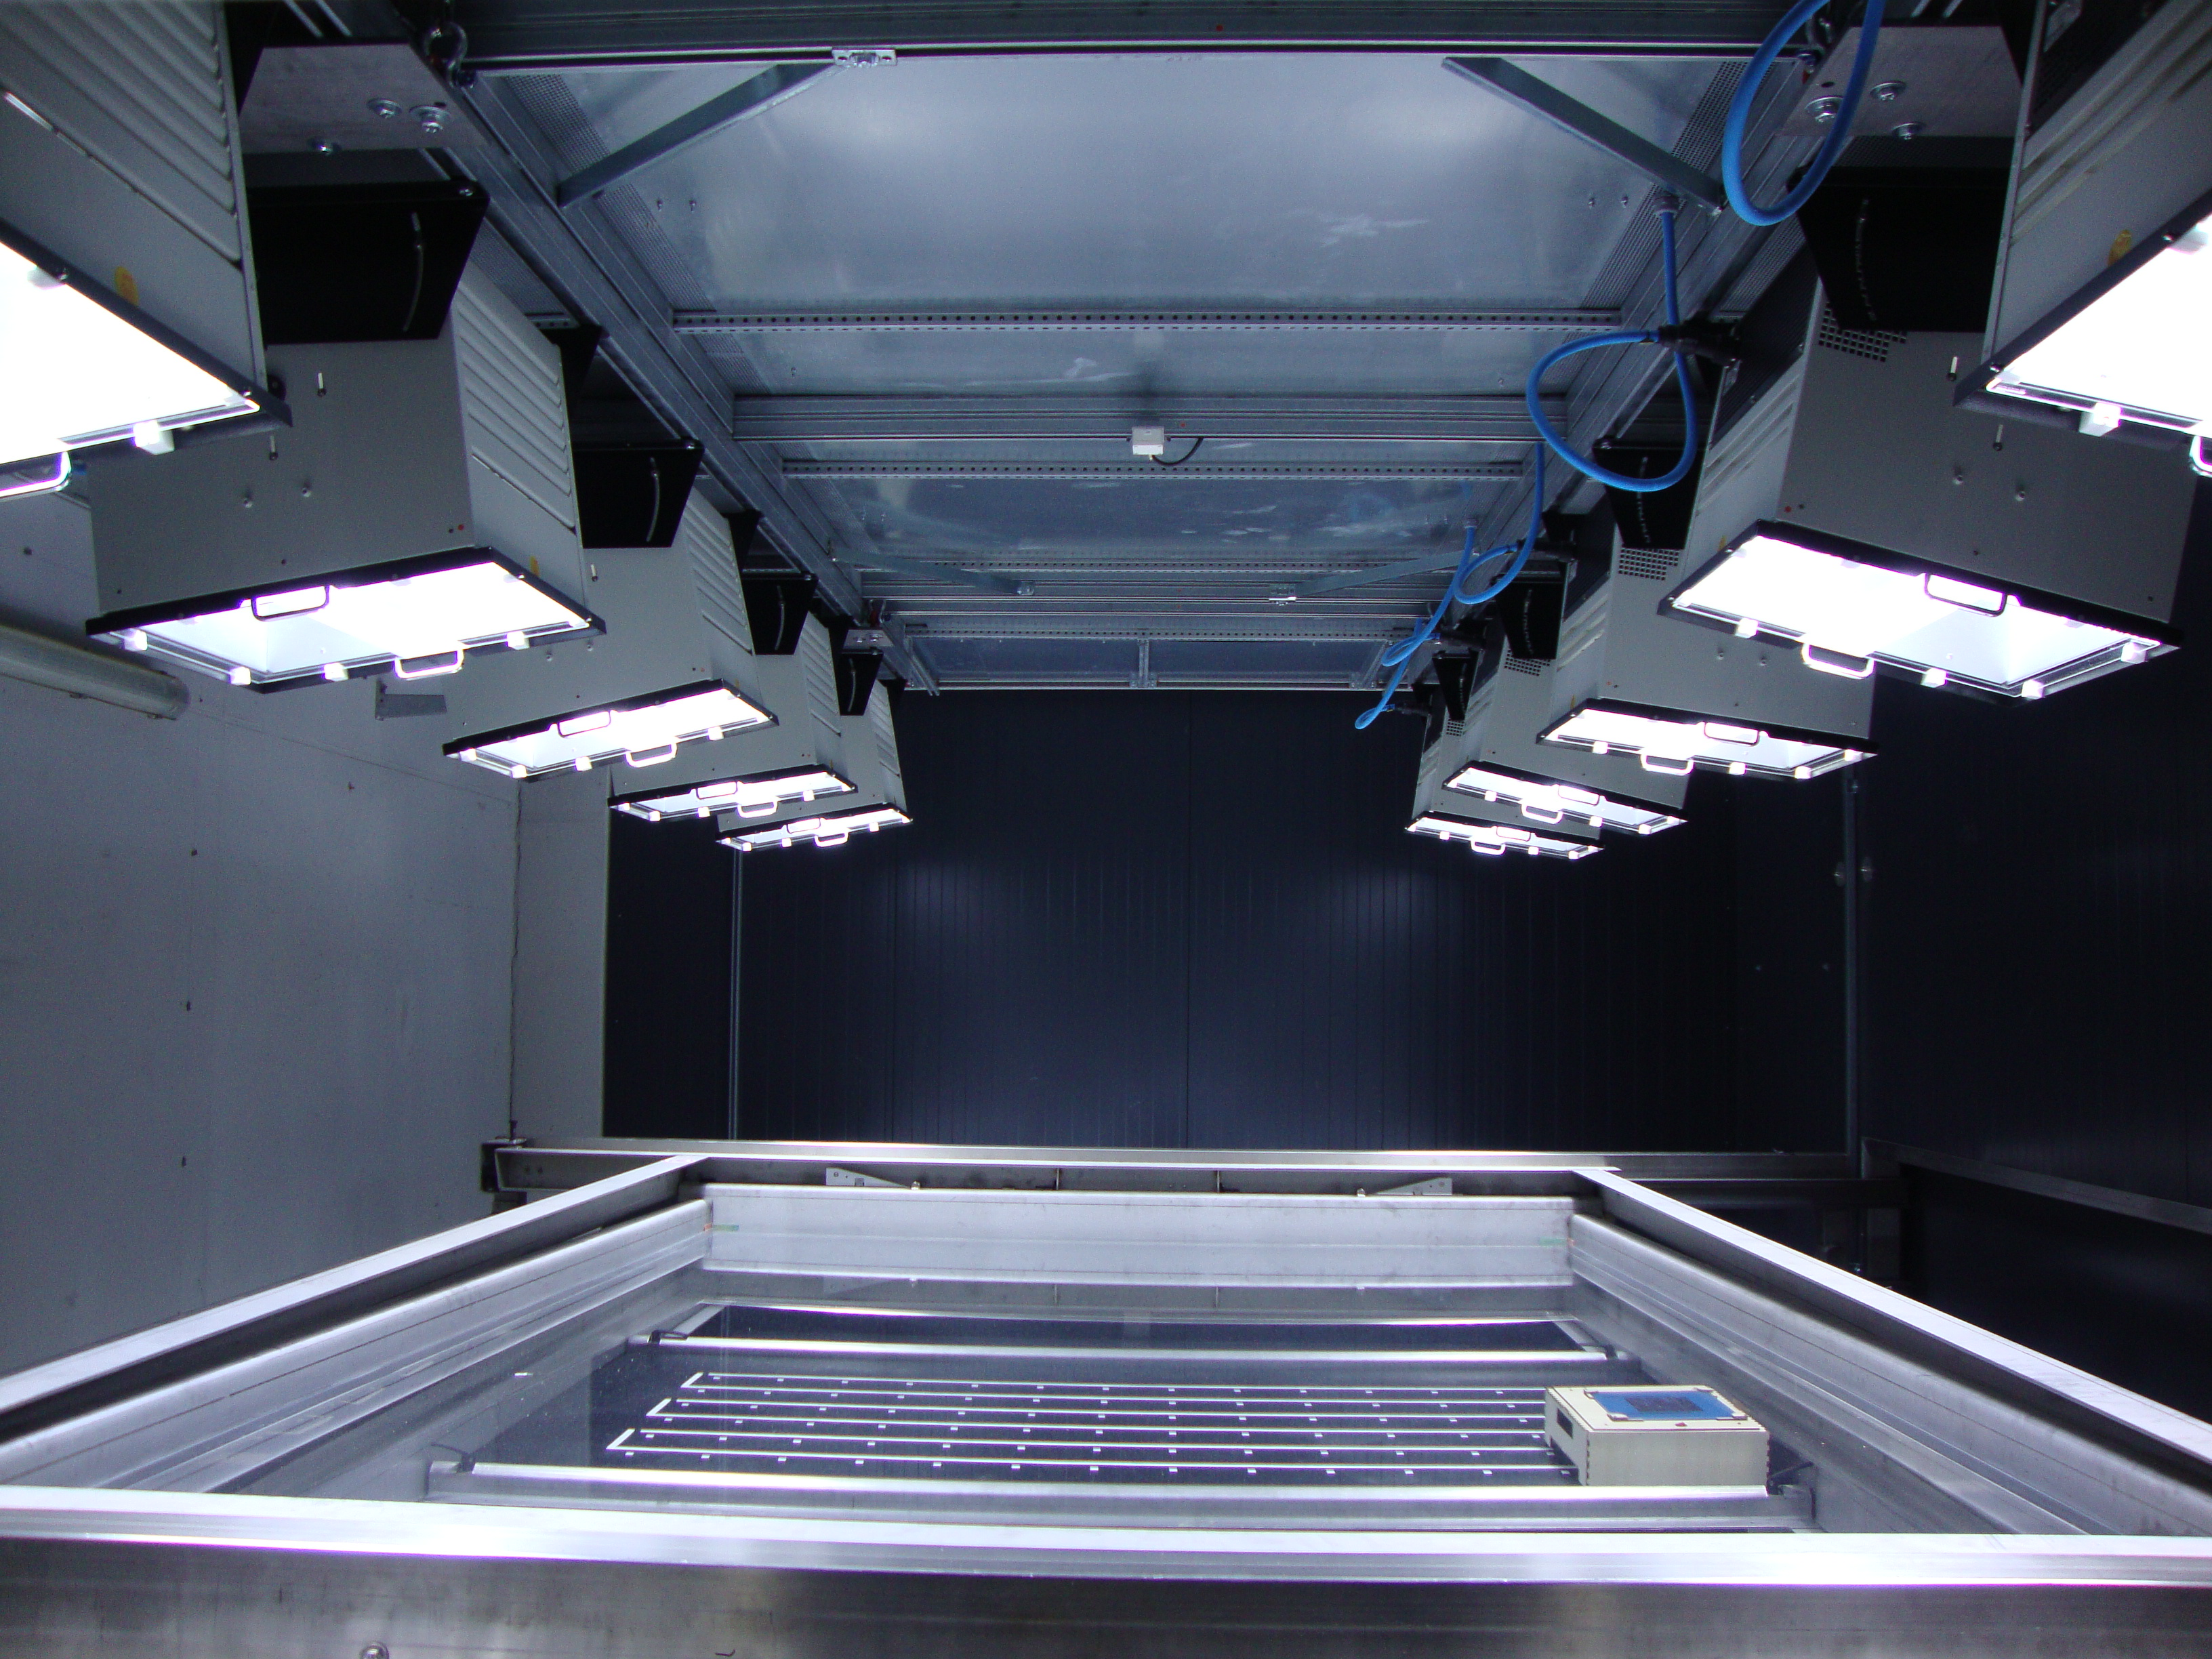
\includegraphics[width=125mm]{img/sunsimulator.jpg}
\caption[Sonnensimulator]{Der Aufbau des Sonnensimulators: Die 10 Metallhalogenoid Strahler befestift an der höhenverstellbaren Aufhängung, der Windkanal und die Prüfebene.}\label{sunsim}
\end{figure}


\section{Normative Anforderungen}\thispagestyle{empty}
Die IEC Norm 60904-9 \cite{norm9} stellt Anforderungen an Sonnensimulatoren. Ein Sonnensimulator wird anhand von 3 Kriterien bewertet: 
\begin{itemize}
\item die spektrale Übereinstimmung mit dem in Tabelle \ref{TabS1} aufgelisteten Wellenlängenbereichen. Zum AM1.5 Referenzspektrum sind durch die großen Schranken erhebliche Unterschiede möglich.
\begin{table}[htbp]
\centering
\begin{tabular}{ | c | c | c |}\hline
{\bf } & {\bf Wellenlängenbereich in nm} & {\bf \% der totalen Einstrahlung}\\ \hline
\hline
1  & 400 - 500 & 18,4 \\ \hline
2  & 500 - 600 & 19,9\\ \hline
3  & 600 - 700 & 18,4\\ \hline
4  & 700 - 800 & 14,9\\ \hline
5  & 900 - 900 & 12,5\\ \hline
6  & 900 - 1100 & 15,9\\ \hline
\end{tabular}
\caption{Spektralle Strahlungsverteilung nach IEC 60904-9}\label{TabS1}
\end{table}
\item die Gleichmäßigkeit der Bestrahlungsstärkeverteilung über die Testfläche
	\begin{equation}
 Non-uniformity (\%) = [\frac{max irradiance - min irradiance}{max irradiance + min irradiance}] \times (100\%)
\end{equation}
\item die zeitliche Stabilität der Einstrahlung.
\begin{equation}
 Temporal (\%) = [\frac{max irradiance - min irradiance}{max irradiance + min irradiance}] \times (100\%)
\end{equation}
\end{itemize}

Tabelle \ref{TabS2} gibt die Anforderungen an, nach denen Sonnensimulatoren in den Klassen A,B und C klassifiziert werden. Die Sonnensimulatorklasse ABB bedeutet eine 0,75- bis 1,25-fache Übereinstimmung in allen in Tabelle \ref{TabS1} angeführten Schranken, eine Homogenität der Einstrahlung zwischen 2\% und 5\% im Messbereich, und eine zeitliche Stabilität zwischen 2\% und 5\%. 
\begin{table}[htbp]
\centering
\begin{tabular}{ | c | c | c | c | c |}\hline
\multirow{2}{*}{Klassifikation} &  Spektrale  &  Örtliche  & {Kurzzeit-}& {Langzeit-}\\
& Übereinstimmung & Homogenität & {stabilität} & {stabilität} \\ 
\hline
\hline
A  & 0,75 - 1,25 & 2 \% & 0,5 \% & 2 \%\\ \hline
B  & 0,6 - 1,4 & 5 \% & 2 \% & 5 \%\\ \hline
C  & 0,4 - 2,0 & 10 \% & 10 \% & 10 \%\\ \hline
\end{tabular}
\caption{Anforderungen an die 3 verschiedenen Simulatorklassen}\label{TabS2}
\end{table}



\section{Theorie Referenzzelle}\thispagestyle{empty}
Eine Solarzelle wandeln die Energie des Lichtes in elektrische Energie um. Eine Referenzzelle ist eine speziell für Messungen kalibrierte Solarzelle. Eine Referenzzellen ist eine genau vermessene Solarzellen, die als Strahlungsmessgerät dient. Wichtig ist, dass die Referenzzelle eine ähnliche spektralle Empfindlichkeit hat wie die zu messenden Zelle bzw. das zu messende Modul
Es gibt verschiedene Solarzellentechnologien. Es gibt kristalline Siliziumzellen und Dünnschichtzellen . Die kristallinen Siliziumzellen werden in monokristalline Zellen und multikristalline Zellen unterschieden. Beide zusammen machen über 80\% des weltweiten Photovoltaikmarktes aus \cite{iea00}. Als Referenzzelle für Messungen werden ausschließlich kristalline Zellen verwendet. 
Eine Siliziumsolarzelle ist eine großflächigen Diode. Die Sperrschicht ist dabei dem Sonnenlicht ausgesetzt. Gelangt ein Lichtquanten in die Sperrschicht kann aufgrund des inneren Photoeffektes ein Elektron/Loch Paar erzeugt werden. Durch das elektrische Feld in der Sperrschicht werden die Ladungsträger getrennt bevor sie kombinieren können. Elektronen bewegen aufgrund ihrer negativen Ladung entgegen der Feldrichtung in die n-Zone. Löcher wandern in Feldrichtung zur Raumladungsfreien p-Zone. Die Leerlaufspannung einer Solarzelle ist kleiner als die Diffusionsspannung, der Spannung über die Raumladungszone, die der Diffusion von Ladungsträgern entgegenwirkt.
\begin{figure}[htbp]
\centering
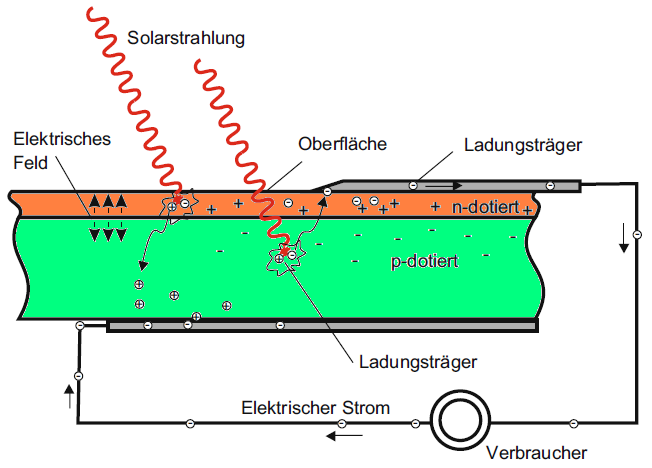
\includegraphics[width=125mm]{img/zelle2.png}
\caption{Der Schematischer Aufbau einer Siliziumsolarzelle. Quelle: \cite{pv}}\label{cell}
\end{figure}


Unbeleuchtet funktioniert die Solarzelle wie eine normale Halbleiterdiode, welche einen Durchlassstrom von p- nach n-Seite fließen lässt, falls eine Spannung von p nach n anliegt. Bei Beleuchtung wird zusätzlich ein Photostrom erzeugt, welcher proportional zur Bestrahlungsstärke und der Zellfläche ist. Das Zweidiodenmodel (siehe Abbildung ~\ref{esb}) besteht daher aus einer Stromquelle, dazu parallel zwei Dioden, einen Parallelwiderstand und einem Serienwiderstand. Der Parallelwiderstand fasst Kurzschlüsse zusammen, die realen Solarzellen am Rand oder an den Korngrenzen auftreten können. Mit dem Serienwiderstand werden alle Spannungsabfälle in der Solarzelle erfasst. Die beiden Dioden bilden die Rekombinations- und Diffusionsprozesse in einer realen Solarzelle ab. Eine ideale Solarzelle hat einen Serienwiderstand von null und einen Parallelwiderstand von unendlich. 
\begin{figure}[htbp]
\centering
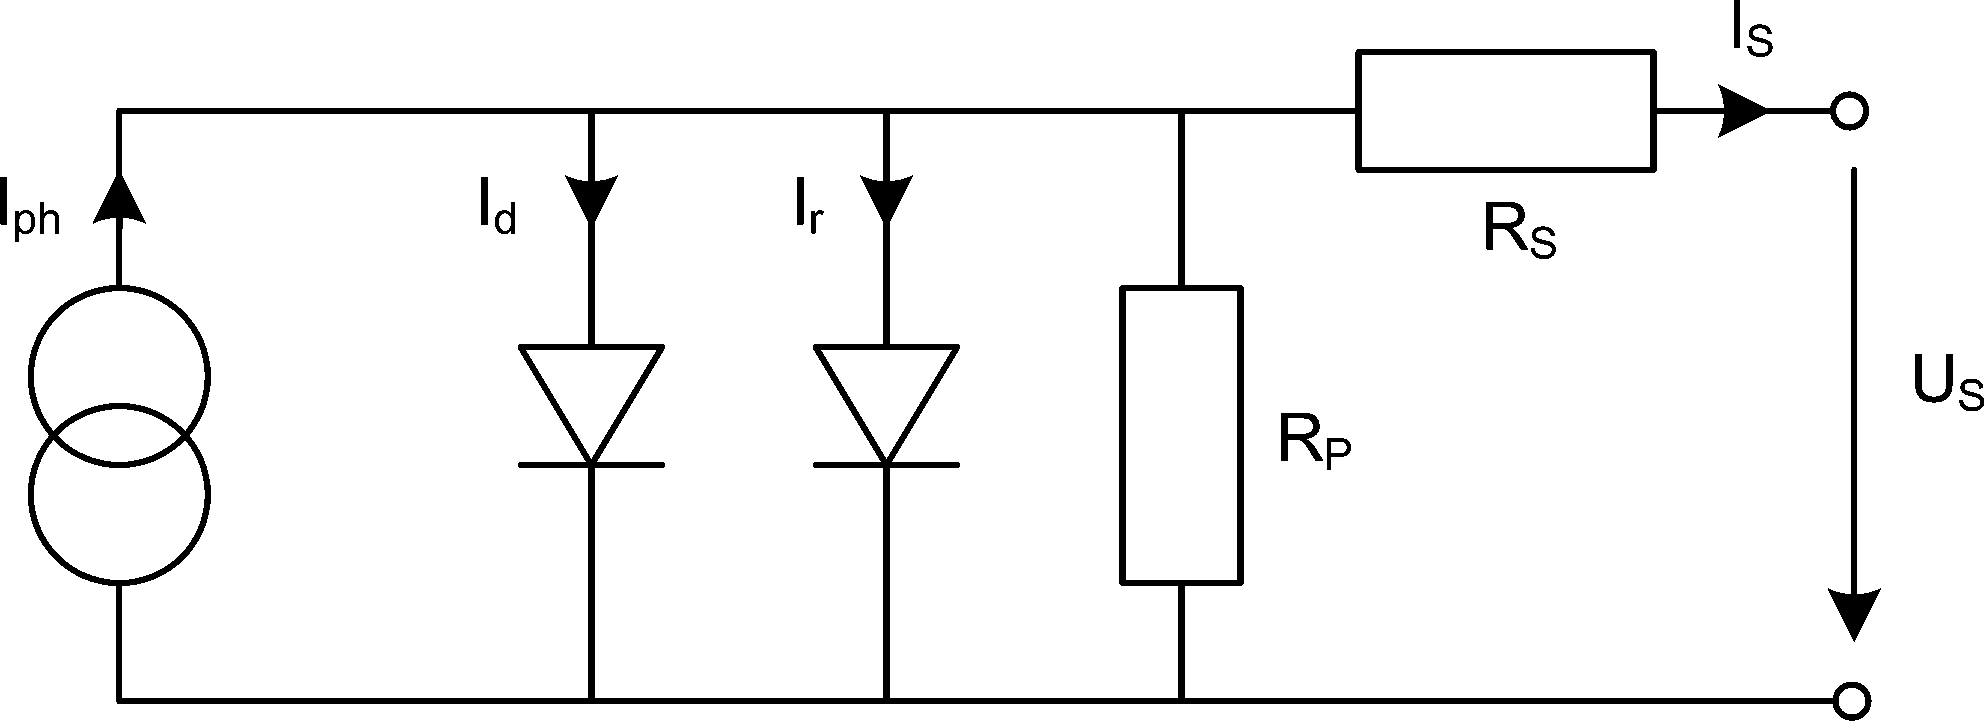
\includegraphics[width=125mm]{img/esb2.png}
\caption{Das Zweidiodenmodell einer Sorlarzelle. Quelle: \cite{pv}}\label{esb}
\end{figure}

Durch den zusätzlichen Photostrom verschiebt (siehe Abbildung ~\ref{kennlinie}) sich die Diodenkennline. Im Leerlauf  bzw. Kurzschlussbetrieb gibt die Solarzelle keine Leistung ab. Der Punkt der Kennlinie mit der maximalen Leistung wird als Maximum Power Point (MPP) bezeichnet.

Der Füllfaktor berechnet sich aus Strom im maximalen Leistungspunkt $I_{mp}$, Spannung im maximalen Leistungspunkt $U_{mp}$, Kurzschlusstrom $I_{sc}$ und Leerlaufspannung $U_{oc}$ zu:
  \begin{equation}
     FF = \frac {I_{mp} U_{mp}} {I_{sc} U_{oc}}
  \end{equation}
Der Füllfaktor ist das Verhältnis der Fläche des Rechteckes mit den Seitenlängen I$_{mp}$ und U$_{mp}$ zu der Fläche des Rechteckes mit den Seitenlängen I$_{sc}$ und U$_{oc}$ (siehe Abbildung \ref{kennlinie}).

\begin{figure}[htbp]
\centering
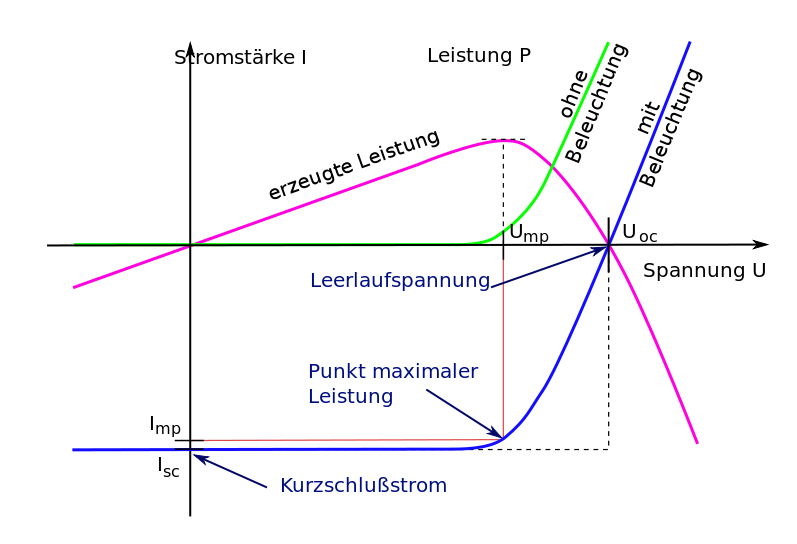
\includegraphics[width=125mm]{img/kennlinie.png}
\caption{Dunkel- und Hellkennlinien. Modifiert nach \cite{kl}}\label{kennlinie}
\end{figure}

Die Kennlinie der Solarzelle ist von der Einstrahlung abhängig (siehe Abbildung \ref{mpp}). Der Kurzschlusstrom ist direkt proportional zur Einstrahlung.
Laut IEC 60891 \cite{norm891} berechnet sich die Einstrahlung aus dem gemessenen Kurzschlussstrom, den STC-Kurzschlussstrom, einen relativen Temperaturkoeffizienten und der Zelltemperatur:
\begin{equation}
G = \frac{1000Wm^{-2}I_{RC}}{I_{RC,STC}} [1 - \alpha_{RC}(T_{RC}-25^{\circ} C]
\end{equation}

\begin{figure}[htbp]
\centering
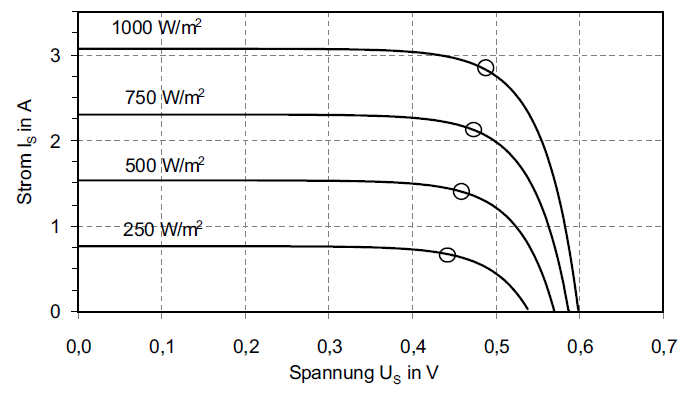
\includegraphics[width=125mm]{img/kennlinien.png}
\caption{Abhängigkeit des MPP von der Einstrahlung. Quelle: \cite{pv}}\label{mpp}
\end{figure}

\begin{figure}[htbp]
\centering
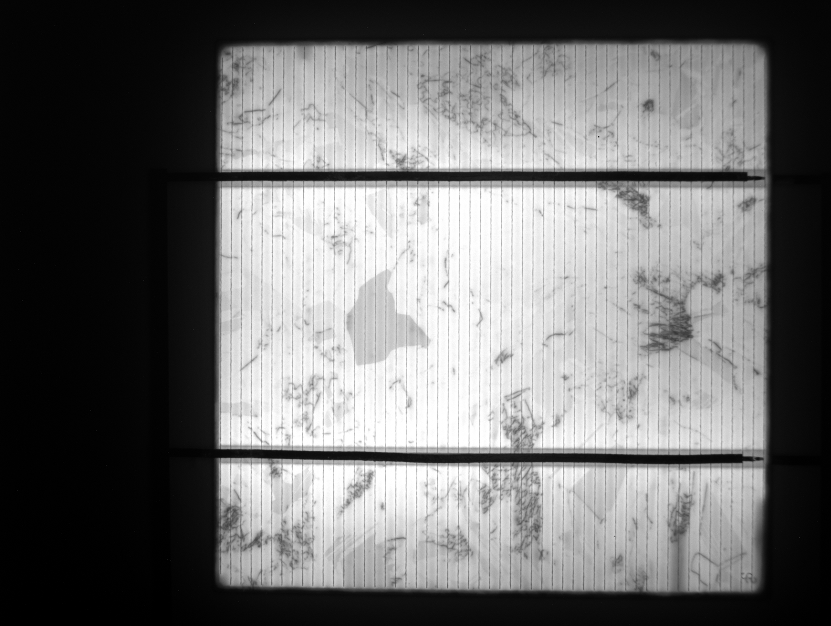
\includegraphics[width=100mm]{img/el.png}
\caption{Eine EL-Aufnahme der verwendeten Messzelle}\label{el}
\end{figure}

\chapter{Entwicklungsprozess}\thispagestyle{empty}

Diese Kapitel beschreibt die Entwicklung des Roboters und ist in 3 Abschnitte gegliedert: das mechanische Design, die Elektronik und die dazugehörige Software.
Dabei wurde teilweise parallel gearbeitet. Zur Entwicklung der Fahrregelung musste die Bodenplatte, aber nicht der Aufbau des Chassis fertig sein. Ebenso musste reichte ein Teil der Elektronik aus, die Messplatinen und die endgültige Stromversorgung war zur Entwicklung der Fahrregelung nicht notwendig. Das hatte den Nachteil, dass die Größe mancher Komponenten (z.B. der Akku) nur abgeschätzt werden konnte, und der Roboter nicht auf eine minimale Größe hin optimiert wurde.

\section{Mechanische Komponenten}\thispagestyle{empty}

Dieser Abschnitt behandelt die Entwicklung der mechanischen Komponenten, diese sind die 4 Mecanumräder und die Chassis des Roboters. Die maximale Bauhöhe ist durch den Windkanal im Sonnensimulator beschränkt, die minimale Bauhöhe ist durch den Durchmesser der Räder gegeben.
Mit der Größe der Messzelle ist auch die minimale Ausdehnung in den beiden anderen Dimensionen festgelegt. Eine weiter Einschränkung beim Design war, dass die Motoren, der Akku und die Elektronik im Inneren des Roboters Platz finden mussten, und der Roboter länger und breiter als die Messzelle wurde (siehe Abbildung \ref{oben}).

\begin{figure}[htbp]
\centering
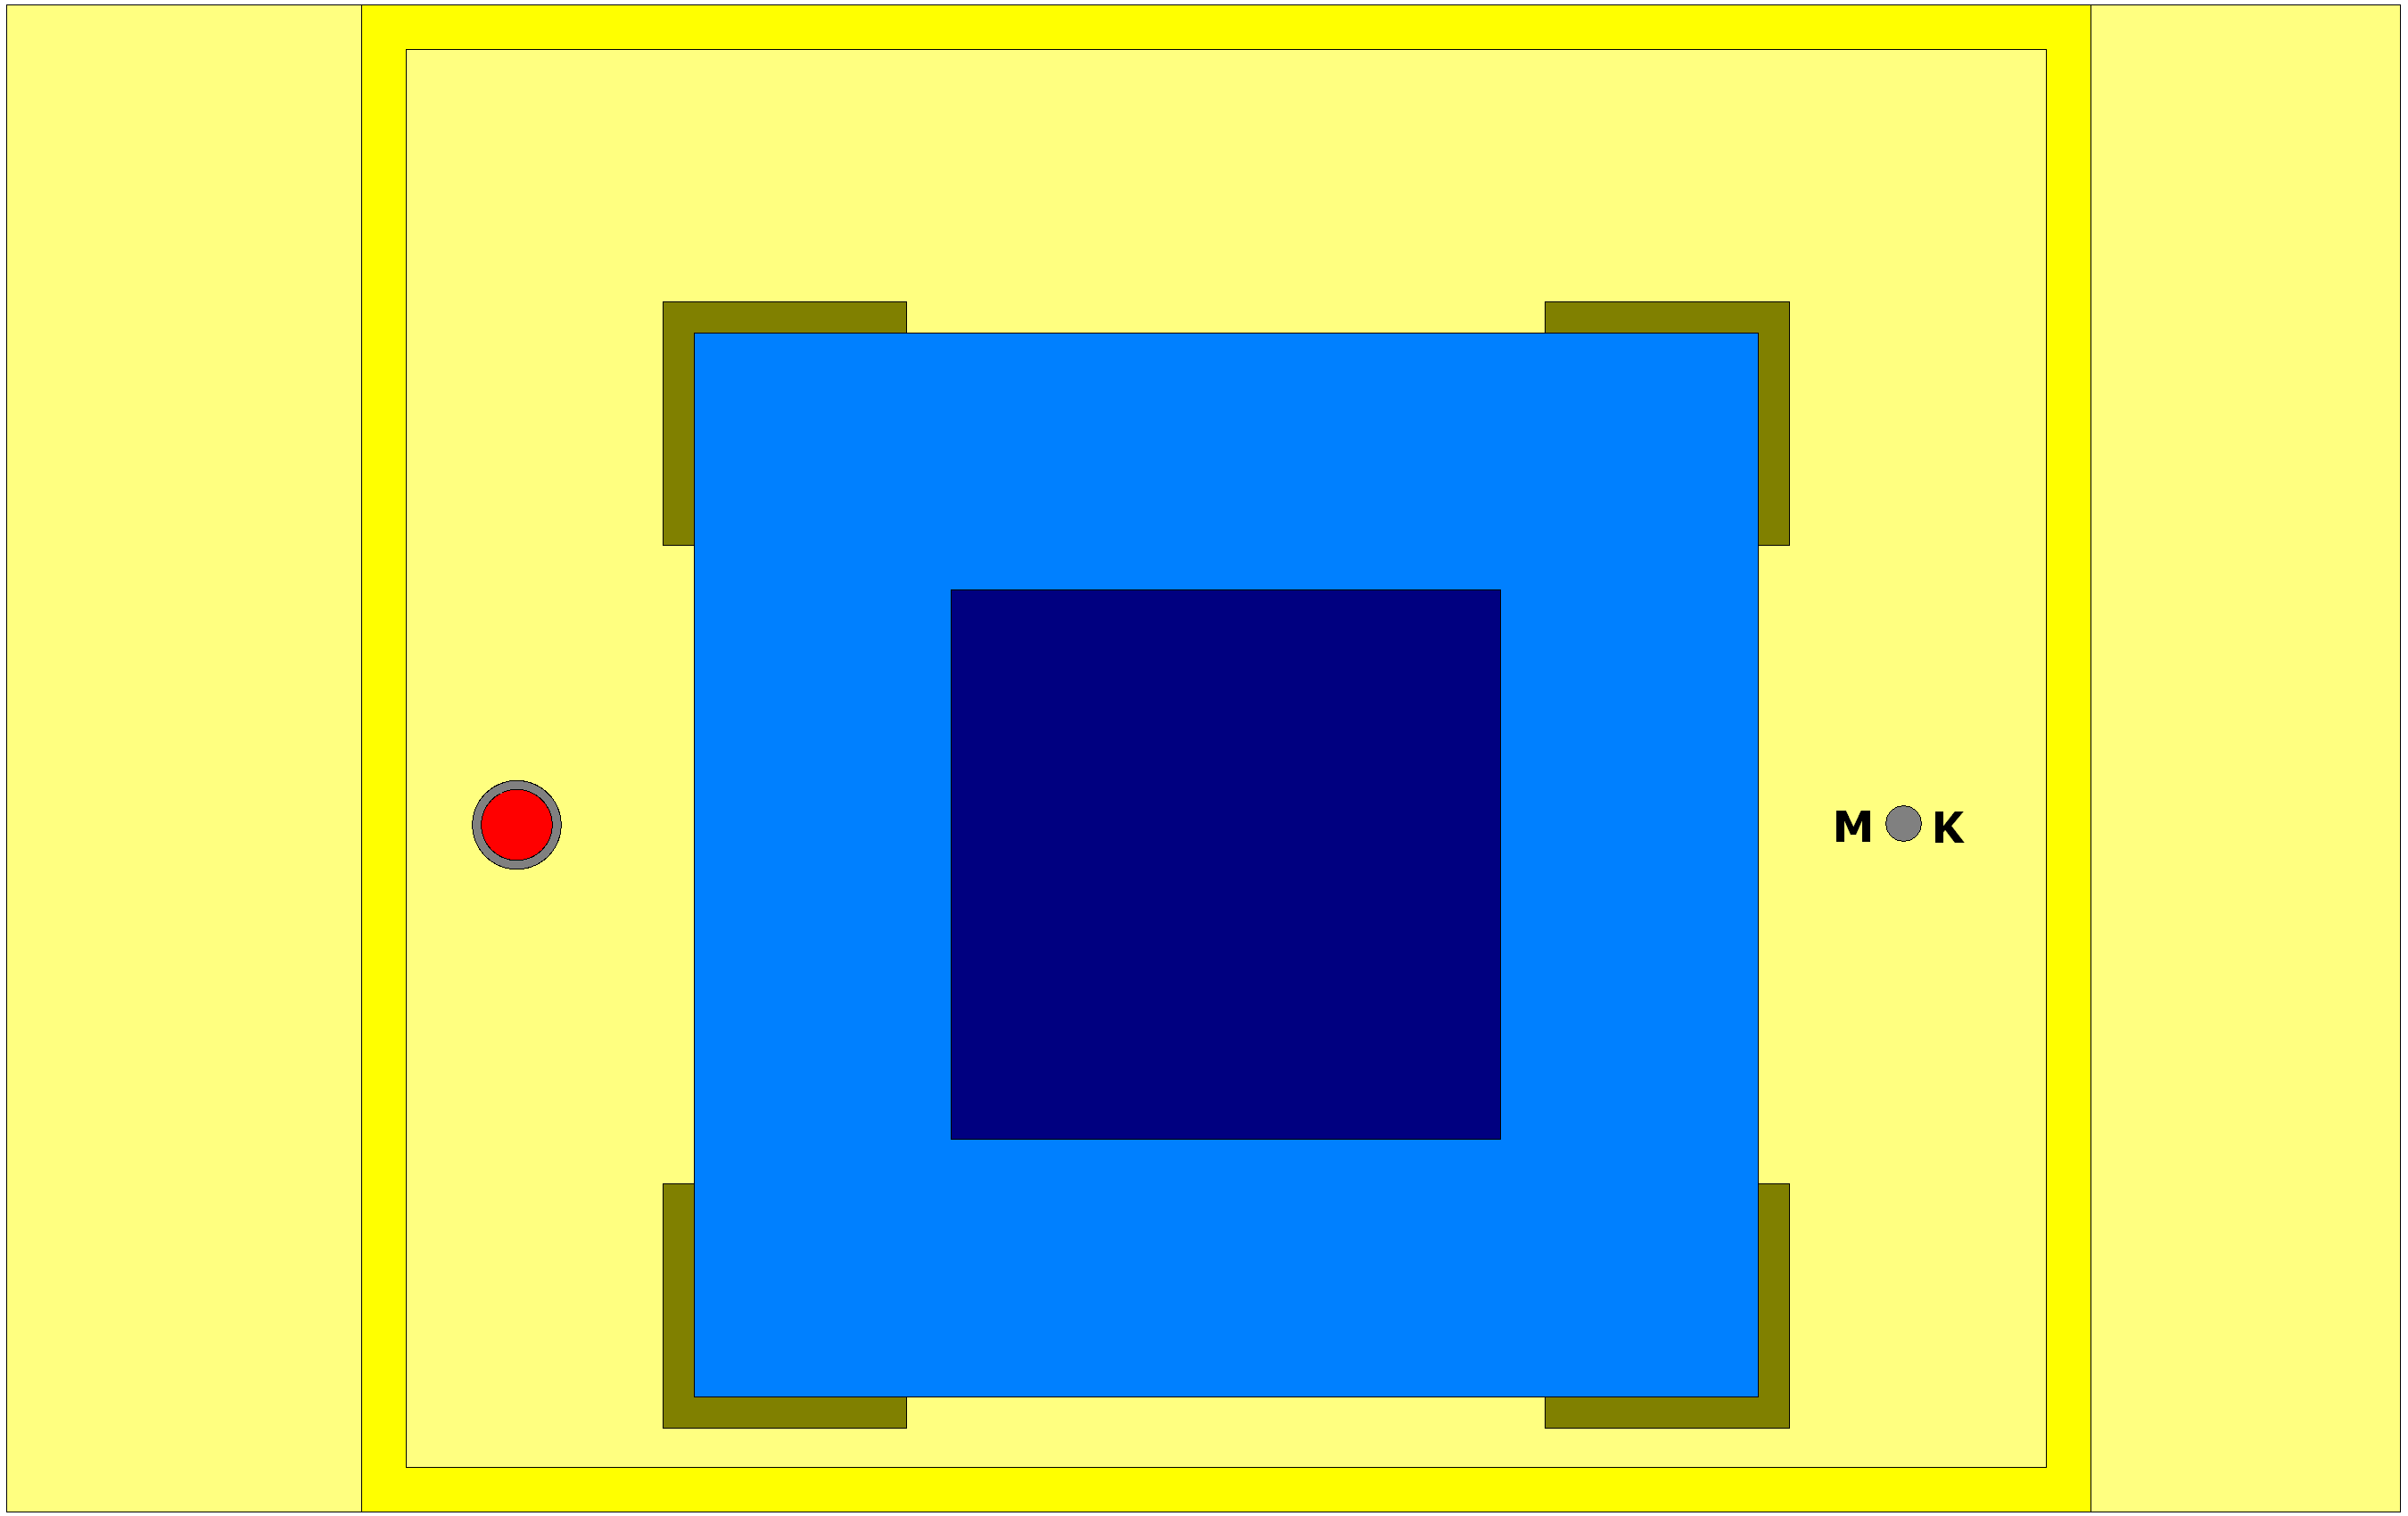
\includegraphics[width=125mm]{img/oben2.png}
\caption{Der Roboter aus der Vogelperspektive}\label{oben}
\end{figure}
  

\subsection{Die Mecanum-Plattform}\thispagestyle{empty}
Mecanum-Räder erlauben einem Fahrzeug, ohne mechanischer Lenkung, sich in jede Richtung zu bewegen. Benannt ist es nach dem schwedischen Unternehmen Macanum, welches dieses Rad 1971 entwickelt hat \cite{mecanum}. 
Jedes Rad wird über einen eigenen Motor angetrieben, und verfügt über eine separate Ansteuerung. Die Räder bestehen aus einer Felge (siehe Abbbildung \ref{rad}), auf der unter einem Winkel von 45 Grad befestigte, ballige Rollen so angebracht sind, die über den Abrollumfang einen exakten Kreis bilden (siehe Abbbildung \ref{rad2}). In die 8 Löcher der Felge werden Kugellager eingeklebt. Jedes der vier Räder besteht aus einer Felge, insgesamt 16 Laufrollen, 8 Kugellager, 8 M4x45mm Schraube, 8 M4 Muttern, sowie 16 M4 Beilagscheiben. 
Das Rad ist mit einer M3 Schraube und einer M3 Mutter an der Motorachse fixiert.
Die Felgen und die Laufrollen wurden mit einem Ultimaker 3D-Drucker gedruckt. 
Die Vorlage namens Mecanum Wheel MK2 stammt von http://www.thingiverse.com/thing:2473, und kann unter der Attribution-NonCommercial-ShareAlike 3.0 Unported Lizenz nicht kommerziell verwendet werden.
Die Laufrollen so angepasst, dass die Mutter bzw. der Schraubenkopf in der Rolle versenkt ist, damit das Rad insgesamt kompakter ist. Zum bearbeiten wurde OpenSCAD, ein 3D-Compiler, verwendet. 

Durch die Schräganordnung der Laufrollen entstehen beim Antreiben eines Rades zwei Kraftkomponenten, eine in Querrichtung und eine in Längsrichtung des Fahrzeuges. Gegeneinander gerichtete Kräfte der einzelnen Räder werden über die Achsen und den Rahmen kompensiert. Die übrigen Kräfte addieren sich zur resultierenden Fahrtrichtung. Auf diese Weise sind durch entsprechendes Ansteuern der einzelnen Räder omnidirektionale Fahrmanöver möglich (siehe Abbildung \ref{fahrman}). So ist es nicht nur möglich den Roboter in Längsrichtung vor und zurück zu bewegen, sondern auch in Querrichtung (normal zur Längsrichtung) zu bewegen, ebenso sind Drehungen am Stand möglich. Damit braucht ein mit Mecanumrädern ausgestatteter Roboter keine Lenkung. Aber es sind zwar vier Motoren notwendig, damit jedes Rad einzeln angesteuert werden kann.   
Die Kugellager sind in den 8 Löchern der Felge verklebt. Zuerst mit Superkleber, allerdings haben sich einige Kugellager im laufe der Zeit gelöst und beeinflussten so das Fahrverhalten negativ. Eine dauerhafte Verbindung von Kugellager mit der Felge ist für den störungsfreien Betrieb des Roboters unumgänglich. 
Zwischen den Rollen und dem Kugellager sorgen Beilagscheiben für einen reibungsarmen Betrieb. 
Die Schrauben der Rollen lösen sich im Betrieb nicht. Die Schraube, welche die Felge an der Motorachse befestig hat, löste sich regelmäßig, bis diese Verbindung mit einem Kleber (Uhu Alleskleber) gesichert wurde.
An den Rollen ist keine Abnützung erkennbar. Die gebrochenen Ringe der Kugellager brachen schon während der Erstmontage, verschlimmert hat sich während der Betriebes nichts.
Es wurde lange mit teilweise defekten Rädern gefahren, ein Messbetrieb war aber dennoch möglich. Insgesamt ist die Mecanum-Plattform eine robuste Lösung für Messroboter.
Die Kugellager sind wartungsfrei. Das wenige UV-Licht, das den ABS-Kunststoff erreicht hat auch nach Monaten noch keine negativen Auswirkungen auf die mechanischen Eigenschaften der Räder.

\begin{figure}
    \subfigure[Vor/Zurück-Fahren]{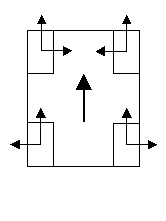
\includegraphics[width=50mm]{img/gerade.png}}
    \subfigure[Das Seitwärtsfahren]{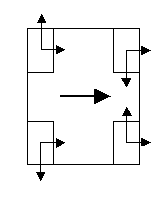
\includegraphics[width=50mm]{img/seitw.png}}
     \subfigure[Drehen am Stand]{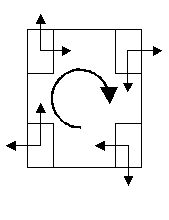
\includegraphics[width=50mm]{img/dreh.png}}
\caption{Einige mögliche Fahrmanöver eines Mecanum-Rad-Roboters}\label{fahrman}
\end{figure} 

\begin{figure}[htbp]
\centering
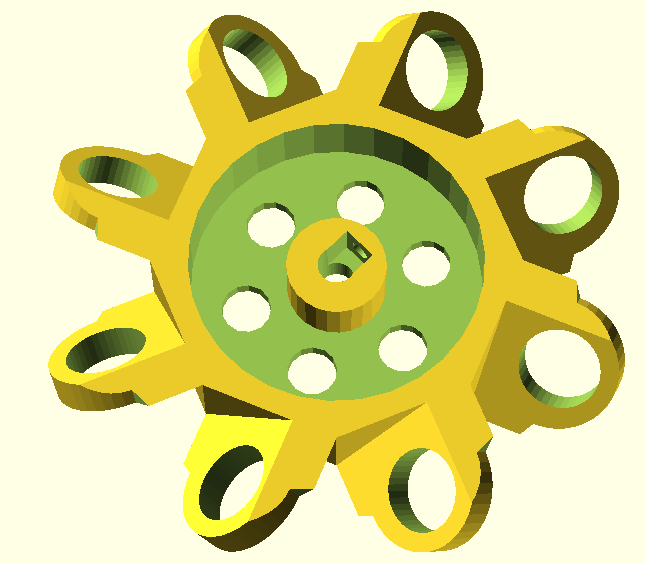
\includegraphics[width=75mm]{img/wheel.png}
\caption{Die Felge des Mecanum Rades}\label{rad}
\end{figure}

\begin{figure}[htbp]
\centering
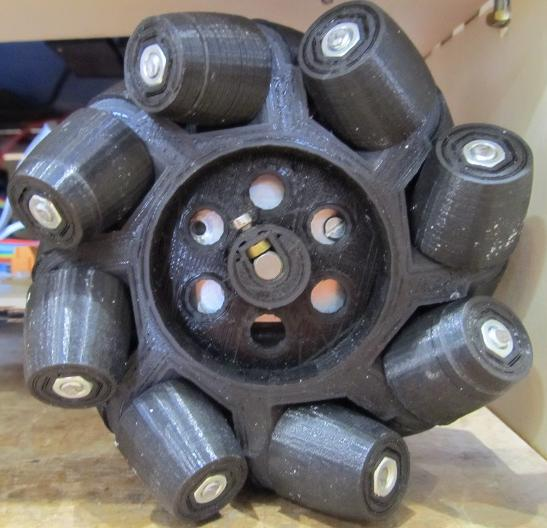
\includegraphics[width=75mm]{img/rad.jpg}
\caption{Ein fertig Rad, montiert am Roboter.}\label{rad2}
\end{figure}


Mit OpenSCAD entsteht ein dreidimensionales Modell eines Werkstückes. Damit fängt eine 3D-Drucker wenig an. Ein 3D-Druck setzt sich aus sehr vielen Liniensegmenten zusammen. Dazu muss das 3D-Modell in einzelne dünne Schichten und einzelne Linien zerlegt werden. Dieser Vorgang wird als "Slicing" bezeichnet. Dazu wurde das Programm pronterface verwendet. Mit OpenSCAD wird zunächst ein stl-File erzeugt, dann produziert pronterface daruas die Fahrbefehle für den 3D-Drucker in Form eines g-Files. Als Druckmaterial wurde ABS (Acrylnitril-Butadien-Styrol) verwendet, welches in einem Temperaturbereich von 215 bis 230 Grad Celsius per Extruder verarbeitet werden kann.    
Die Druckzeit pro Rolle betrug 20 Minuten. Insgesamt mussten 64 Rollen gefertigt werden. Die Druckzeit pro Felge betrug etwa drei Stunden, der Roboter benötigte 4 Felgen. Es gibt insgesamt zwei verschiedene Felgentypen, mit nach links oder nach rechts geneigten Rollen. 
Dazu kommen noch vorbereitende Testdrucke bis die einzelnen Komponenten optimiert waren und der Drucker befriedigend Ergebnisse lieferte. 
Nach dem Drucken mussten die Teile nachbearbeitet werden.  Die Löcher für die Kugellager mussten per Hand passend gefeilt werden. Beim  Einsetzen der Kugellager brachen manche der Halterungen. Mit Klebstoff konnten die Kugellager auch in die gebrochenen Halterungen eingebaut werden. Die dauerhafte Haltbarkeit dieser Konstruktion ist allerdings mit einem Fragezeichen behaftet.

\subsection{Chassis}\thispagestyle{empty}

\noindent Das Chassis wurde aus Sperrholz gefertigt. Dieses Material wurde gewählt weil es leicht zu bearbeiten, robust und UV-beständig ist. Das Design wurde mit QCAD entwickelt. QCAD ist ein 2-dimensionales CAD Programm. 
Die Abmessungen des Chassis wurde im Wesentlichen abgestimmt auf: \begin{itemize}
\item Den Durchmesser und der Breite der Mecanum Räder, die innerhalb des Chasis liegen, damit die Räder vor der UV Strahlung geschützt sind, kein Einfluss (Beschattung oder Reflexionen) auf die Messzelle besteht.
\item Die Größe der Motoren.
\item Den Arduino-Mikrocontroller , die Motorsteuerelektronik und die Messelektronik
\item Den Akku zur Stromversorgung, die dazugehörende Akku Spannungsüberwachung 
\item Die Abmessung der eingekapselten Solarzelle.
 \end{itemize}

Das Chassis besteht aus der Bodenplatte, den Seitenwänden und der oberen Abdeckung mit der Aufnahme für die Messzelle (siehe Abbildung \ref{gehause}). In der Bodenplatte sind Bohrlöcher zur Befestigung der Motoren und für die Montage der Sensorarrayplatine an der Unterseite vorhanden. Zusätzlich gibt es zwei rechteckige Löcher für die Verbindungskabel zur Sensorarrayplatine. Die beiden Seitenwände sind zur Verringerung des Luftwiderstandes geneigt (siehe Abbildung \ref{robo3d}). (Und um dem Roboter den Look eines Schuhkartons zu nehmen.)
\noindent Die Einzelteile wurden mit einem Lasercutter aus einer Sperrholzplatte geschnitten. Damit eine zukünftige Wartung problemlos möglich ist, wurde der Aufbau verschraubt ausgeführt. 
Die Motoren sind an die Bodenplatte angeschraubt, damit ein Austausch möglich ist. Auch die einzelnen Räder, wie auch die Rollen lassen sich bei Bedarf austauschen. 
Die Messzelle ist am Roboter oben befestigt.


\begin{figure}[htbp]
\centering
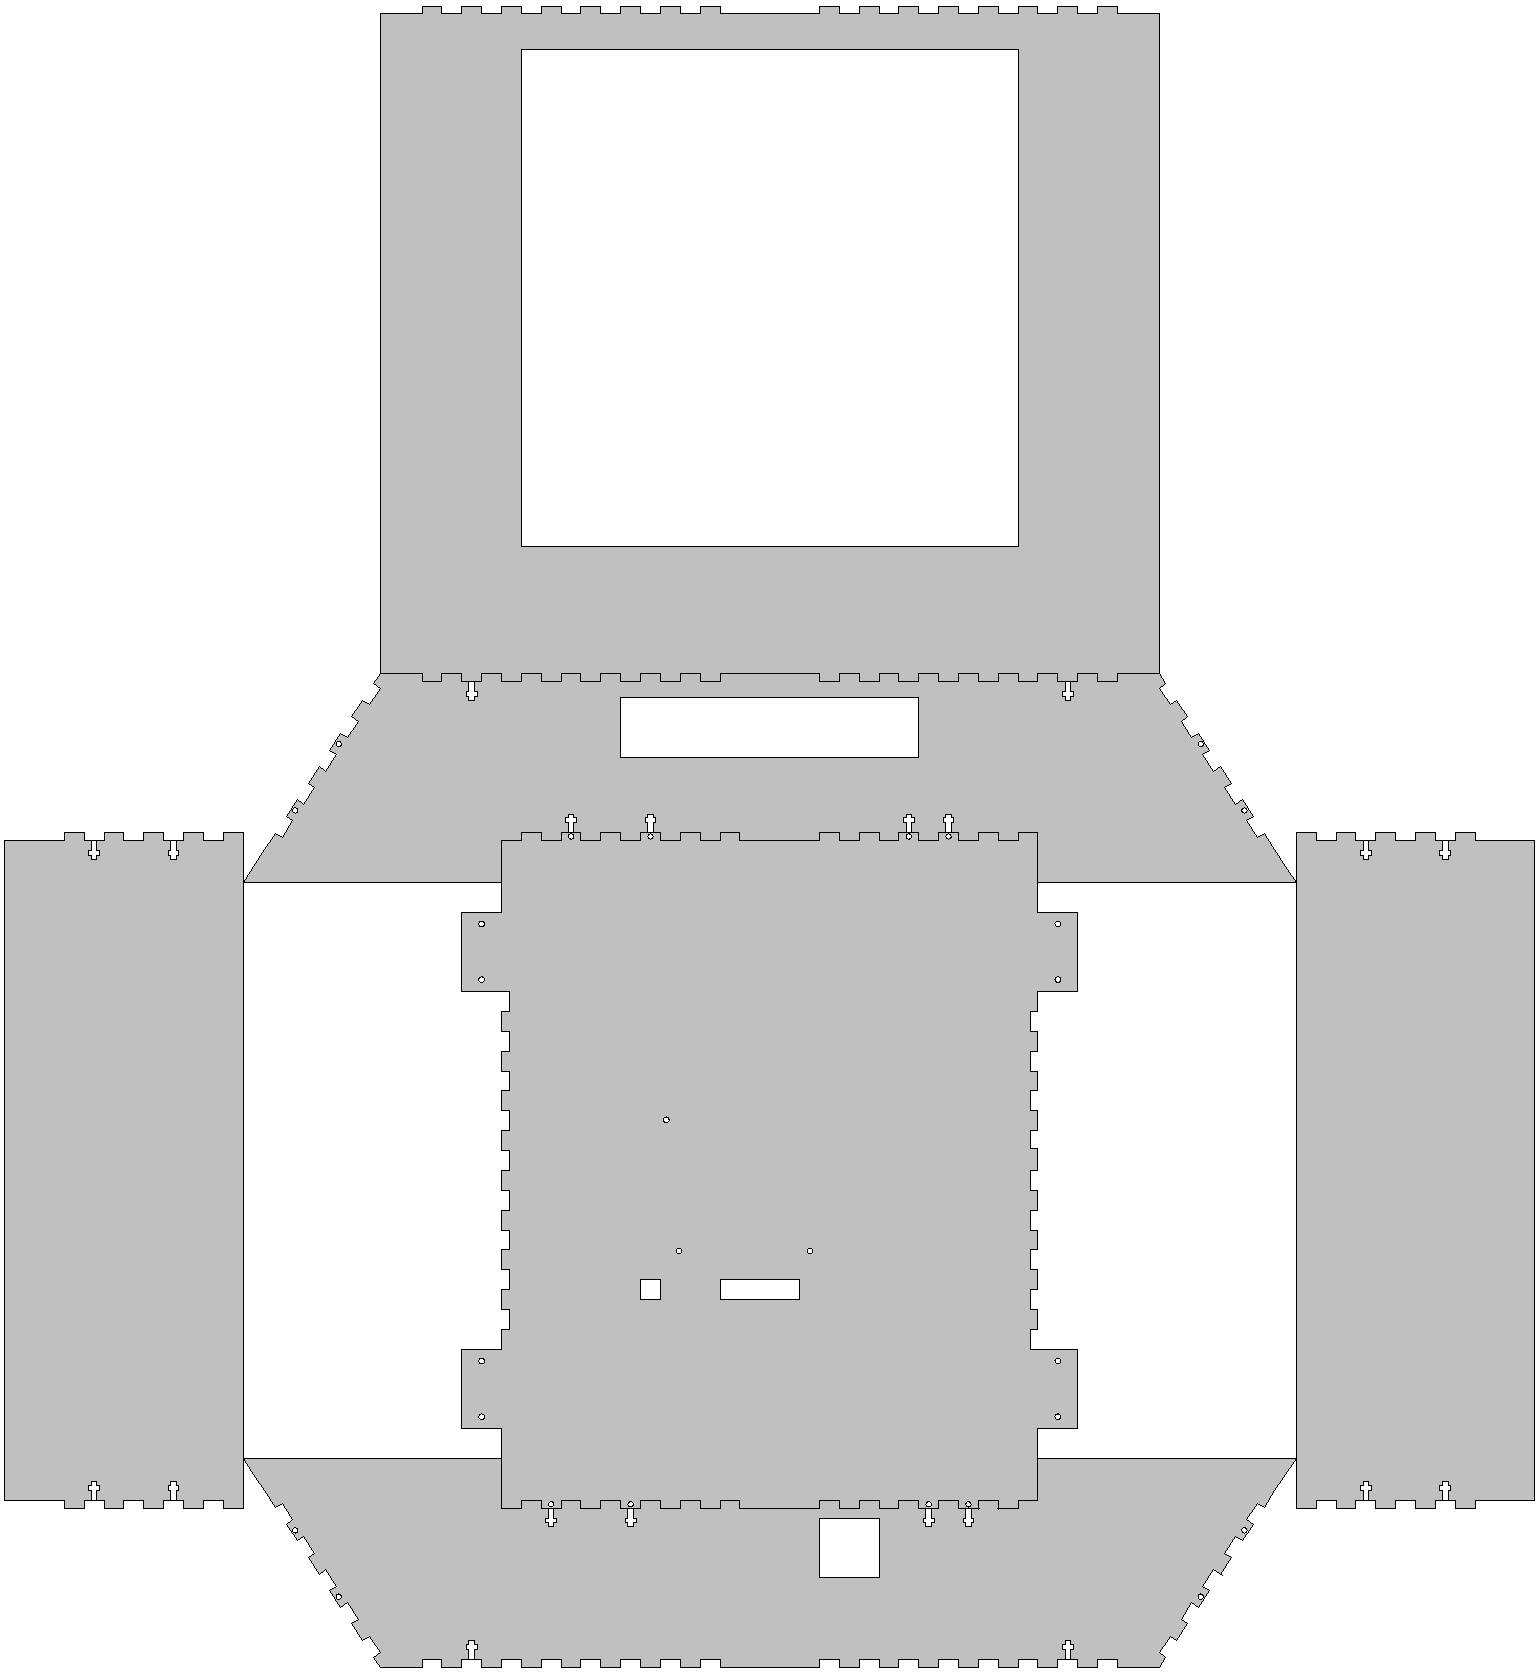
\includegraphics[width=125mm]{img/gehause3.png}
\caption[Chassis]{Die Schnittvorlage des Chassis}\label{gehause}
\end{figure}

\begin{figure}[htbp]
\centering
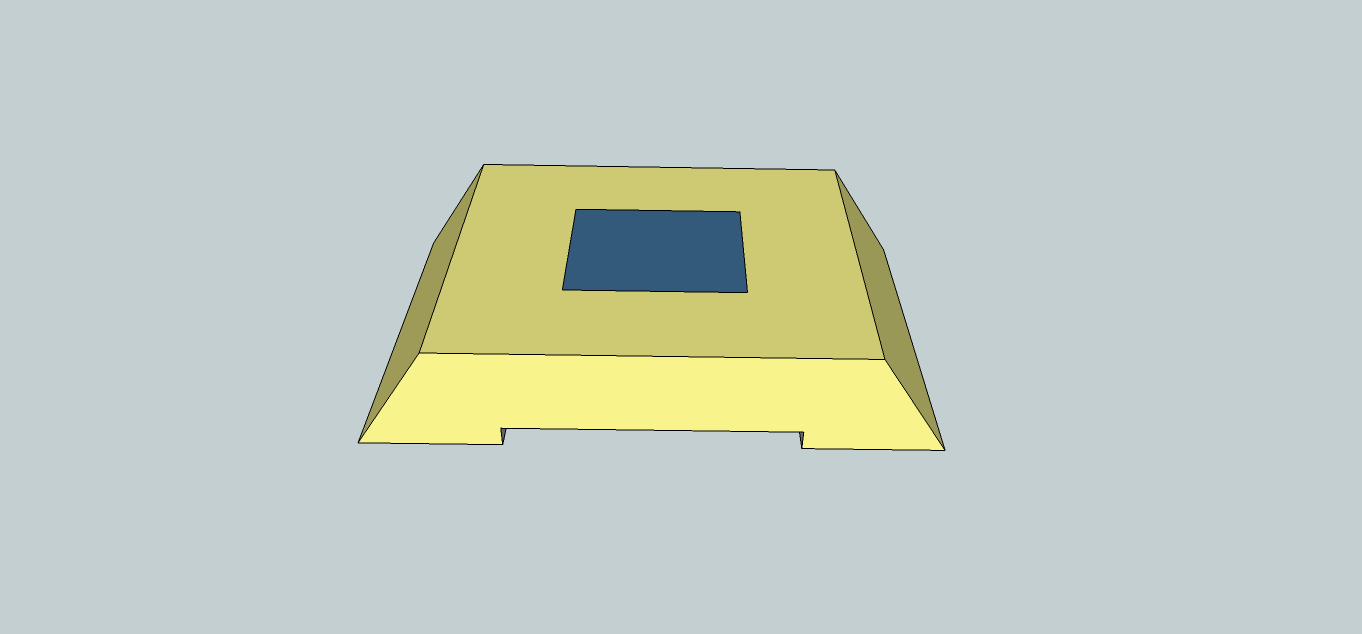
\includegraphics[width=125mm]{img/robo3d.png}
\caption[Chassis]{Ein 3D-Modell der Chassis}\label{robo3d}
\end{figure}


\section{Elektronik}\thispagestyle{empty}

Dieser Abschnitt beschreibt die Entwicklung der Elektronik. Die Funktionalität wurde auf verschiedene Module aufgeteilt. Das erleichterte die Platzierung der Elektronik innerhalb des Messroboters, die parallele Entwicklung von Elektronik und Software, sowie den Austausch von Komponenten im Fehlerfall. 
Das Gehirn des Roboters ist ein Arduino Mega 2560 Mikrocontroller Board. Darauf aufgesteckt ist ein sogenanntes Shield, eine selbst entwickelte Platine, das die $\pm$5V Spannungsversorgung, die Schnittstellen zu den anderen Platinen und einen SD-Karten Einschub beheimatet.
Es gibt 3 Messplatinen, eine für den Kurzschlussstrom der Messzelle, zwei für Temperaturmessungen. Eine Platine überwacht den Ladezustand des Akkus. Die Steuerung der vier Motoren ist auf einer Platine zusammengefasst.
Die einzelnen Komponenten sind wie in Abbildung \ref{elek} auf der Bodenplatte angeordnet.
\begin{figure}[htbp]
\centering
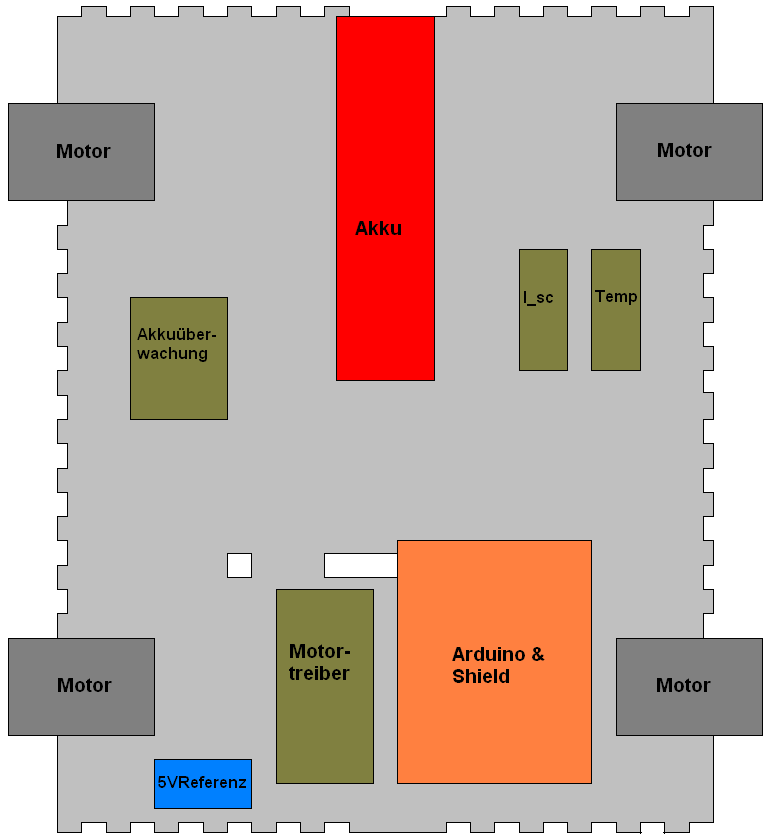
\includegraphics[width=100mm]{img/bodenplatte.png}
\caption{Die Anordnung der Elektronik auf der Bodenplatte im Roboter}\label{elek}
\end{figure}
 
\subsection{Motorensteuerung}\thispagestyle{empty}

Die Motorplatine \ref{hbridge2} besteht aus zwei integrierten H-Brücken-Bausteinen (IC1, IC2), einer 16 poligen Buchse und fünf zweipoligen Buchsen für die Stromversorgung und den Anschluss der vier Motoren. Bei den integrierten H-Brücken-Baustein handelt es sich um einen NJM2670 \cite{njm}, welcher zwei H-Brücken in einem Baustein vereint, zusätzlich verfügen diese Bausteine über eine interne Logik, welche Kurzschlüsse über die Brücke unmöglich macht.
Die Drehzahl der Motoren wird mit Pulsweitenmodulation variiert. Dabei ist es wichtig, dass die Transistoren in der Brücke schnell genug schalten können. Die PWM-Ausgänge des Arduino arbeiten mit einer Frequenz von etwa 500Hz \cite{pwm}.
Die Gleichspannungsmotoren sind Getriebemotoren mit der Bezeichnung RB 35, und einem Übersetzungsverhältnis von 1:200. Die maximale Versorgungsspannung wurde mit 12V angegeben. Die Leerlaufdrehzahl beträgt bei 12V Versorgungsspannung 20 Umdrehungen pro Minute.
Der Roboter wird mit einem Lithium-Ionen-Akku versorgt. Die Spannung beträgt, abhängig vom Ladezustand zwischen 16,4V und 15,0V. Damit die 12V-Motoren nicht überlastet werden, wird bei der Pulsweitenmodulation ein maximales Tastverhältnis von 50\% eingehalten.
 

\begin{figure}[htbp]
\centering
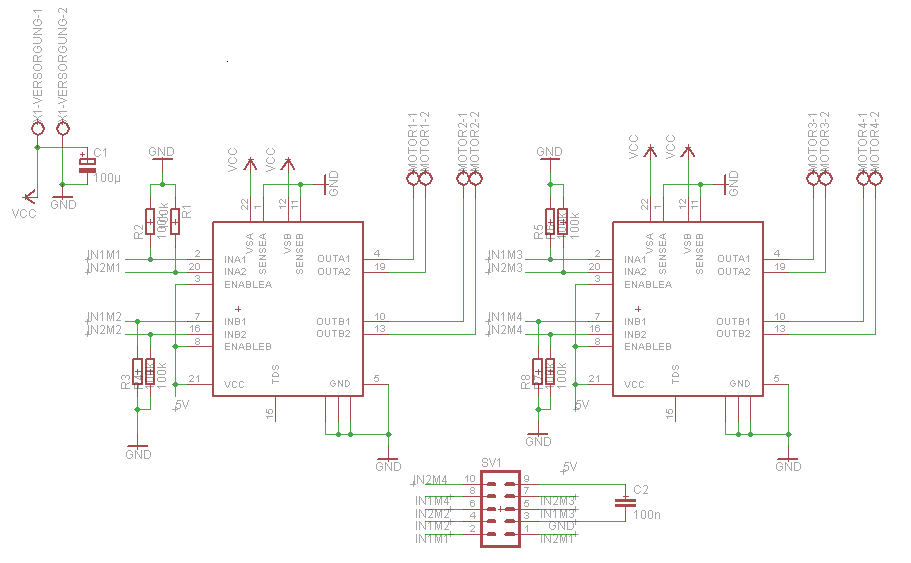
\includegraphics[width=150mm]{img/HBrucke.png}
\caption{Der Schaltplan der Motortreiberplatine.}\label{hbridge2}
\end{figure}

\begin{figure}[htbp]
\centering
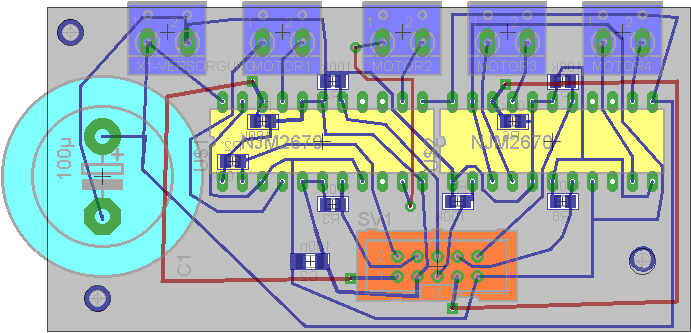
\includegraphics[width=125mm]{img/hdrive.png}
\caption{Das Layout der Motortreiberplatine.}\label{hbridge2}
\end{figure}

\subsection{Optische Sensoren}\thispagestyle{empty}
Die optische Sensorik dient der Positionsbestimmung. Der Roboter bewegt während der Messung auf Holzplatten, die aus Gründen, welche unten genauer erläutert werden, schwarz sind, der Roboter orientiert sich an einer aus geraden Teilstücken bestehenden weißen Linienfolge. 
Als Sensor wurde ein CNY70 \cite{cny} verwendet. Der CNY 70 ist ein Reflexionssensor, bestehend aus einer Infrarot-Led und einem Phototransistor in einem kompakten 7x7x6 Millimeter Gehäuse. Die LED sendet Infrarotlicht mit einem Maximum bei 950nm aus, welches an einer nahen Fläche reflektiert wird, und einem Phototransistor ansteuert. (siehe Abbbildung \ref{cny}) Der Phototransistor verfügt über einen Tageslichtfilter. Damit können Unterschiede des Reflektionkoeffizienten gemessen werden. Das Messprinzip funktioniert bei eienem Abstand von wenigen Millimetern.  Deshalb sind die Markierungen weiß auf schwarzen Untergrund. Eine Anordnung von neun solcher Sensoren in einem 3-mal-3 Array kann sowohl vertikale als auch horizontale Linien sowie Ecken erkennen. Zusätzlich gibt es einen 10. Sensor, der die Stopmarkierungen für die Messungen erkennt.
Die neun Sensoren sind im Rastermaß 15,2 mm (= 0,6 Zoll) angeordnet. Der Stopsensor hat einen Abstand von 40,6 mm (= 1,6 Zoll) zu dem Sensorarray. 
Der Strom durch die LEDs ist mittels Potentiometer einstellbar. 
Die Platine ist zweiseitig ausgeführt, allerdings sind alle Bauteile an der Unterseite der Platine montiert, bis auf die OPVs in SMD-Ausführung. Das ursprüngliche Layout wurde um folgende zwei Änderungen modifiziert:
- Auf die Steuerleitung des Transistors wurde vergessen. Da es noch freie Pins am 16-poligen Stecker gab, wurde diese Verbindung mittels Draht hergestellt.
- Die Platine wird mit der 5 Volt Versorgung der restlichen Elektronik versorgt, welche konstanter als die 7805-Variante ist, und um Probleme mit zwei verschiedenen 5 Volt Versorgungen zu vermeiden. Dazu wurde der ursprünglich vorgesehene 7805 ausgebaut, und eine weiterer freier Pin des 16-poligen Steckers verwendet.

\begin{figure}
    \subfigure[Gehäuse und Innenleben]{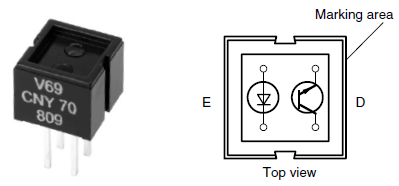
\includegraphics[width=0.49\textwidth]{img/cny1.png}}
    \subfigure[Funktion]{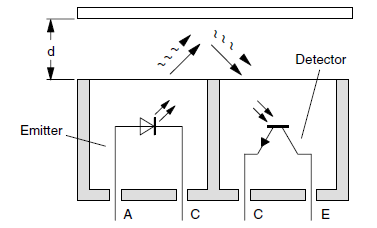
\includegraphics[width=0.49\textwidth]{img/cny2.png}}
\caption{Der Bauteil CNY70} \label{cny}
\end{figure} 

\begin{figure}[htbp]
\centering
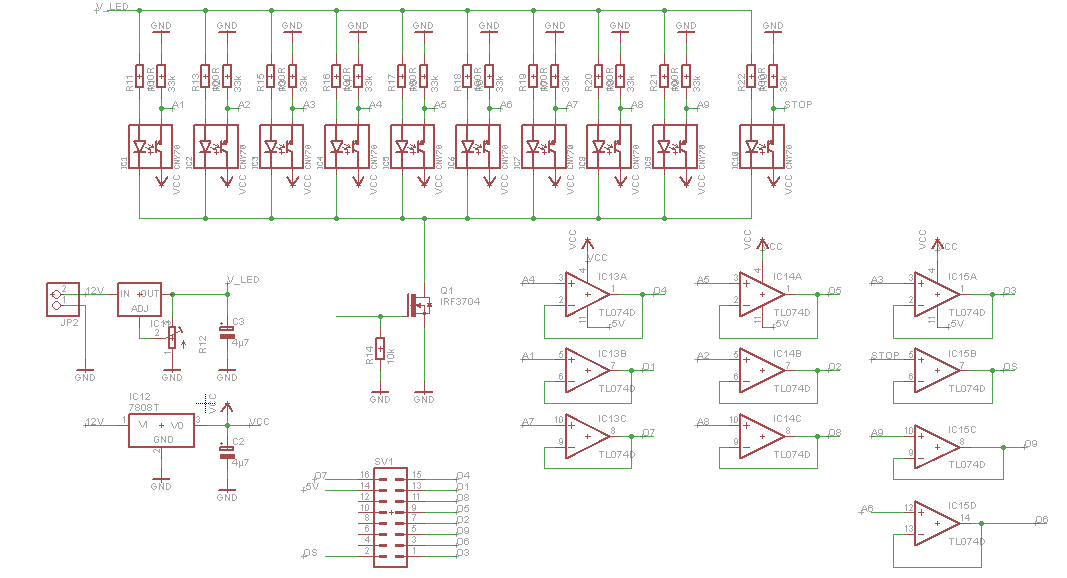
\includegraphics[width=125mm]{img/array.png}
\caption{Der Schaltplan des Sensorarrays.}\label{array}
\end{figure}
Die LEDs sind parallel geschaltet und werde alle über den Feldeffekttransistor Q1 des Typs IRF530 geschaltet.
Der Strom durch die LEDs wird mit einem LM317 geregelt. Da der Widerstand als Potentiometer ausgeführt ist lässt sich der Strom einstellen. Trotz einer nicht konstanten Versorgungsspannung kann so einer konstanter STrom geliefert werden. Um das analoge Messsignal der Phototransistoren nicht zu belasten, werden die analogen Photosignale über einen Spannungsfolger geführt. Die OPVs benötigen allerdings eine symmetrische Versorgung mit $\pm$5 V. Beide Spannungen werden über den Stecker geliefert.
Es gibt weiteren Stecker mit 2 Pins, welche die Spannungsversorgung mit 16 Volt und GND sicherstellt. 
Die Platine verfügt um drei Bohrlöcher mit jeweils drei Millimeter Durchmesser zu Befestigung.
Anschlüsse: Es ist eine 16-polige Leiterplattenbuchse für die Analogsignale, 5V-Versorgung, und des Digitalsignal zum Schalten des FET. Des Weiteren ist ein zweipoliger Stiftstecker für die Stromversorgung mit der Akkuspannung vorhanden.

\begin{figure}[htbp]
\centering
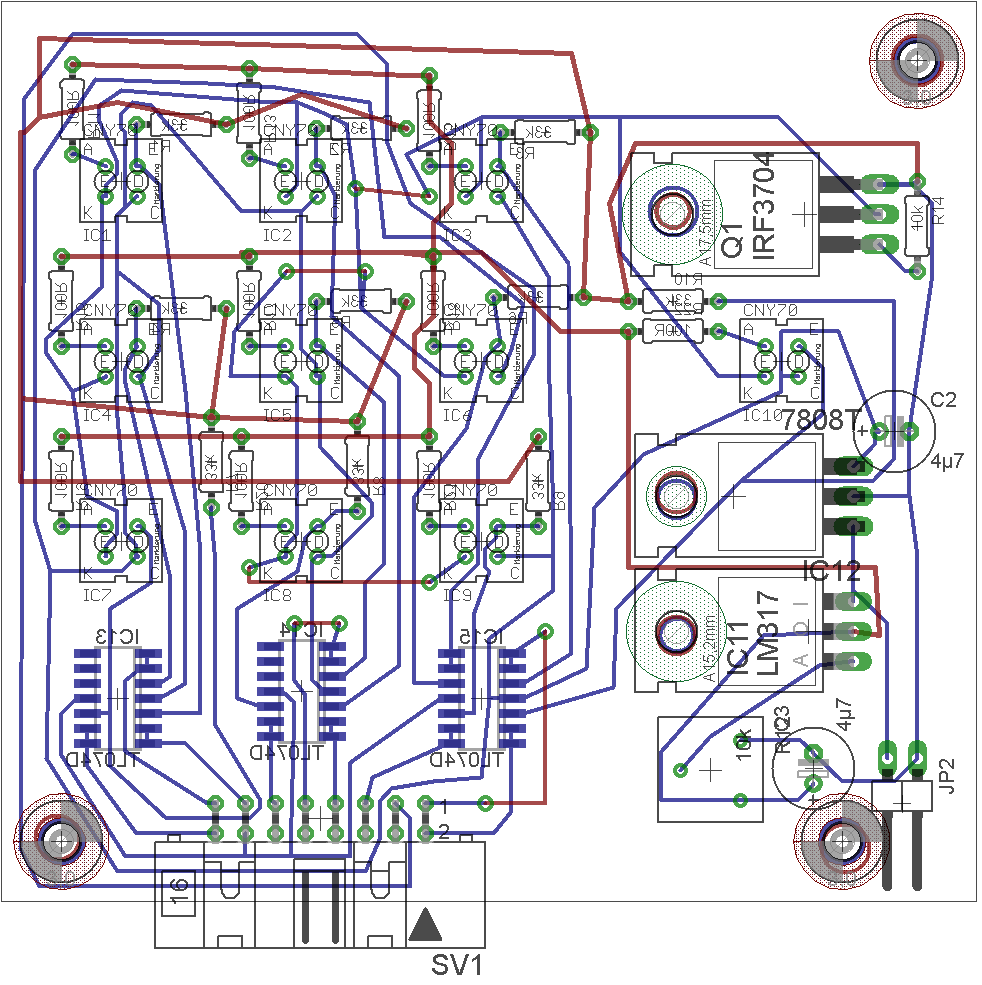
\includegraphics[width=100mm]{img/array21.png}
\caption{Das Layout des Sensorarrays. Die optischen Sensoren sind rosa markiert.}\label{array2}
\end{figure}

\begin{figure}[htbp]
\centering
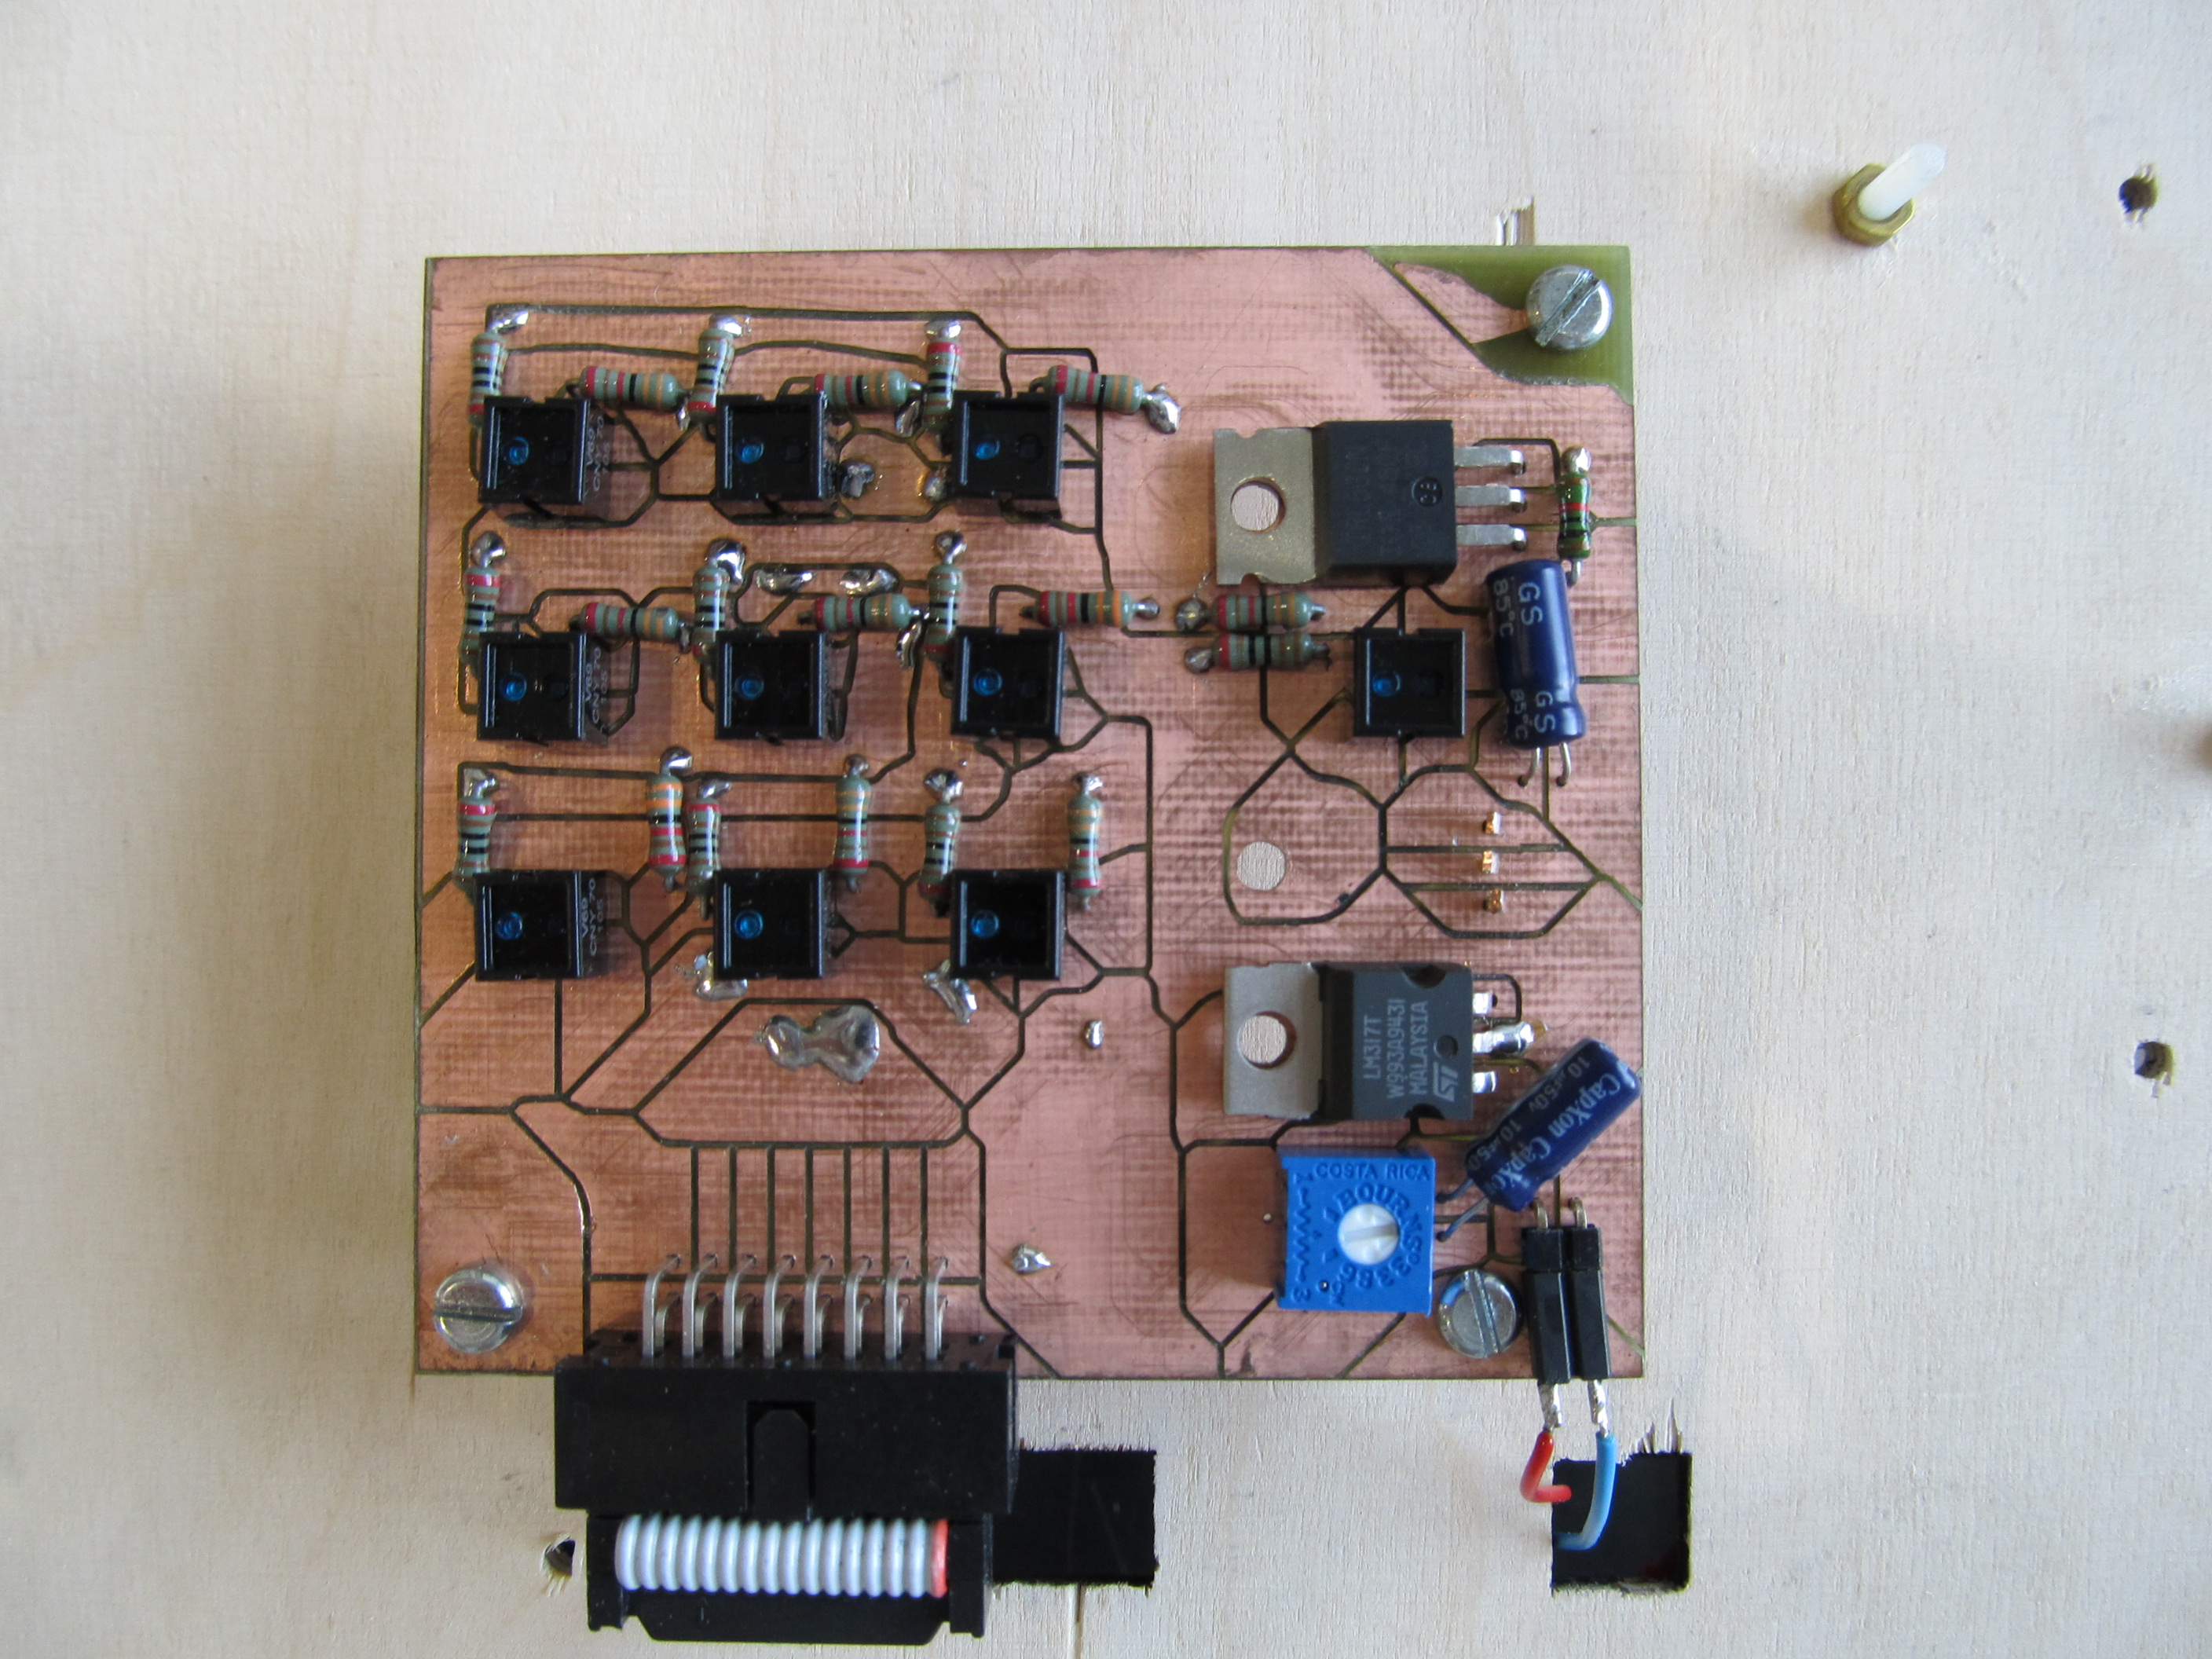
\includegraphics[width=125mm]{img/sensor_array.jpg}
\caption{Die fertige Platine des Senorarrays.}\label{array3}
\end{figure}



\subsection{Spannungversorgung}\thispagestyle{empty}
Die Energie zum Betrieb des Roboters stammt aus einem Kokam 14,6V 4000mAh Litihum Lithium-Polymer-Akkumulator. Es wird empfohlen vor jeden Messzyklus den Akku zu laden. Ein voller Akku reicht für mehr mehrere Stunden Dauerbetrieb. Der Akku ist mit einer im Anschlusskabel integrierten Schmelzsicherung geschützt. Zum Laden des Akkus muss der Akku vom Roboter abgesteckt werden und an das Ladegerät angeschlossen werden. Zum Schutz vor Kurzschlüssen ist der Akku mit einer im Anschlusskabel integrierten Schmelzsicherung gesichert. Da zum Laden der Akku aus dem Roboter entfernt und an das Akkuladegerät angeschlossen werden muss, könnte versehentlich der Akku kurzgeschlossen werden. Zum Laden wird ein Ultramat 16 S verwendet, der über einen Balanceranschluss verfügt, und somit alle vier Zellen des Akkus auf die gleiche Spannung lädt. 
Der Akku kann mit bis zu 200A belastet werden, allerdings liegt der maximale Strom aller 4 Motoren und der restlichen Elektronik liegt bei einem Ampere. Die Motoren werden direkt mit der Akkuspannung versorgt. Die Versorgungsspannung schwankt zwischen der vollen Akkuspannung 16,4V und 15V nach mehr als 10 Messfahrten.
Die 5 Volt Versorgung des Mikrocontrollers wurde mit einem RECOM R-785.0-1.0 DC-DC Konverter gelöst. Er ist pinkompatibel zu einem 7805, allerdings mit einer größeren Dicke, und bietet die Vorteile einer geringen Verlustleistung und einer sehr genauen Ausgangsspannung. 
Der Ladezustand der einzelnen Zellen des Akkus wird mit einer eigens dafür entwickelten Schaltung überwacht. Sollte die Spannung einer Zelle unter 3,3V sinken, wird die Stromversorgung zum Roboter mittels FET unterbrochen, und ein akustisches Warnung ausgegeben. Damit wird eine Tiefentladung verhindert, was zu einer irreversiblen Schädigung und einem Kapazitätsverlust führen kann. Eigentlich könnte der Akku bis zu 2,7V pro Zelle entladen werden.
Die Analog-Digitalwandlung des Arduino benötigt eine Referenzspannung, entweder die Versorgungsspannung, was jedoch zu ungenau ist. Als Spannungsreferenz wird daher ein LT1021 5V Präzisionsspannungsquelle verwendet. Da dieses Bauelement nachträglich hinzugefügt wurde, ist es auf einer eigenen kleinen Platine untergebracht.

\begin{figure}[htbp]
\centering
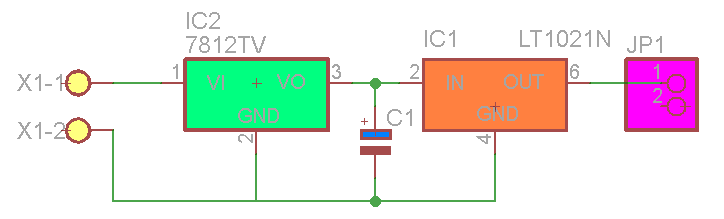
\includegraphics[width=100mm]{img/refu.png}
\caption{Die Schaltung der 5V Referenzspannung.}\label{refu}
\end{figure}

\begin{figure}[htbp]
\centering
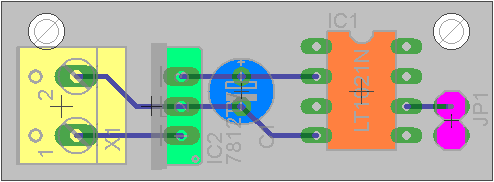
\includegraphics[width=100mm]{img/refu2.png}
\caption{Das Platinenlayout der 5V Referenzspannung.}\label{refu2}
\end{figure}

 
\subsection{Mikrokontroller}\thispagestyle{empty}
Der Arduino Mega 2560 ist ein Mikrocontroller-Board. Es ist eine Open-Source Elektronikentwicklungsplattform und richtet sich an Elektronikneulinge wie auch an Profis. Den Mikrocontroller des Arduino-Boards bildet ein ATmega2560 der Firma Atmel. Dabei handelt es sich um einen 8-Bit-Mikrocontroller.  Er läuft mit 16 MHz Taktfrequenz und besitzt 256 KByte Flash, wovon 8 KByte für den bootloader verwendet werden, für den Programmcode, 8 KByte SRAM, sowie 4 KByte EEPROM.  Es verfügt über 54 digitale I/O Pins, davon können 15 als PWM-Ausgänge verwendet werden. Weiters gibt es 16 analoge Eingänge die über einen 10-Bit Analog-Digital-Wandler verfügen.
Eine USB Schnittstelle ist zur Programmierung und Kommunikation vorhanden.
Der Mikrocontroller arbeitet mit einer Versorgungsspannung von 5V. Grundsätzlich kann die Stromversorgung über die USB Schnittstelle erfolgen. Für einen beweglichen Roboter ist diese Option jedoch nicht praktikabel. Es besteht auch die Möglichkeit über eine Buchse eine Versorgungsspannung von 7 bis 12 Volt anzulegen, der Akku liefert aber eine höhere Spannung. So wird aus der Akku-Spannung mittels DC-DC Konverter
eine stabile 5 Volt Spannung gewonnen. Diese 5 Volt werden direkt mit dem 5 Volt Pin des Arduino-Boards verbunden. Die 5-Volt Spannungsversorgung befindet sich auf dem Shield (der Aufsteckplatine). Dabei handelt es sich um einen kompakten DC-DC Konverter.

\begin{figure}[htbp]
\centering
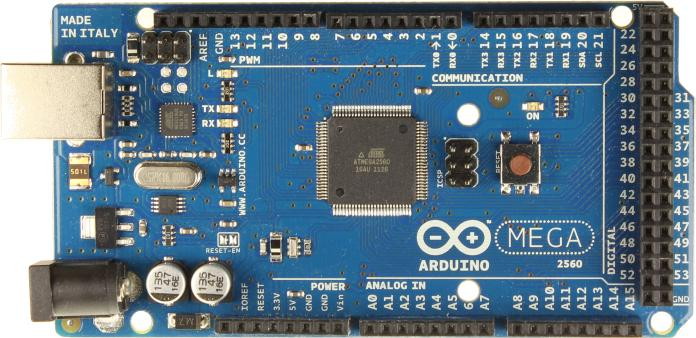
\includegraphics[width=100mm]{img/ArduinoMega2.jpg}
\caption[Arduino Mega 2560]{Arduino Mega 2560}\label{ardu}
\end{figure}

\subsection{Strommessung}\thispagestyle{empty}
Der Kurzschlussstrom der Messzelle wird mit einer eigenen Platine gemessen. Der Strom wird mittels Spannungsabfall an einem 10m$\Omega$ Shunt-Widerstand gemessen. Zu berücksichtigen ist allerdings auch der Spannungsabfall auf der Verbindung von der Zelle zum Shunt-Widerstand.
Die Zelle ist über ein 25cm langes Kabel mit dem Durchmesser von 4 mm$^2$, ein 7cm langes Kabel mit dem Durchmesser von 6mm$^2$, und zwei Bananenstecker mit der Messplatine verbunden. Der Widerstand dieser Verbindung zusammen mit dem Messshunt beträgt etwa 40 m$\Omega$, was bei einem Kurzschlusstrom von etwa 5 A zu einem Spannungsabfall von 200mV führt. Der gemessene Strom ist damit nicht mehr der Kurzschlussstrom. Abbildung \ref{kenn2} zeigt die Widerstandsgerade im Vergleich zur Kennline einer Zelle.

\begin{figure}[htbp]
\centering
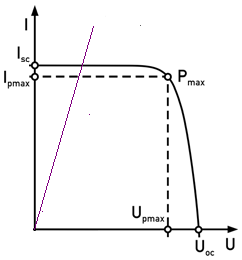
\includegraphics[width=50mm]{img/kenn2.png}
\caption{Einfluss des Widerstandes im Messpfad auf den gemessenen Strom}\label{kenn2}
\end{figure}

\begin{figure}[htbp]
\centering
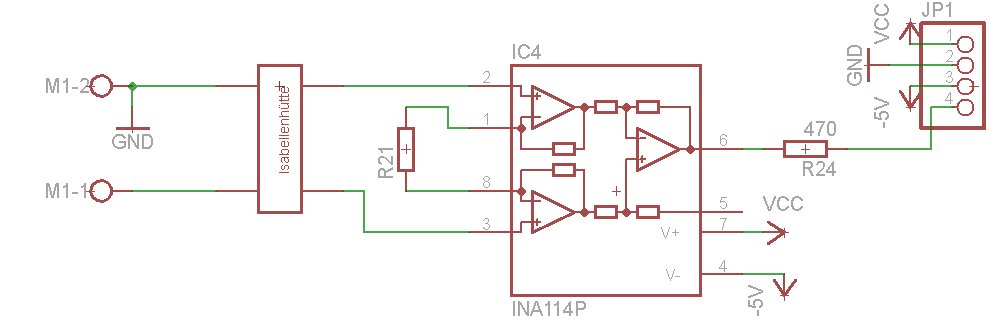
\includegraphics[width=100mm]{img/i1.png}
\caption{Die Schaltung zur Strommessung}\label{i1}
\end{figure}

\begin{figure}[htbp]
\centering
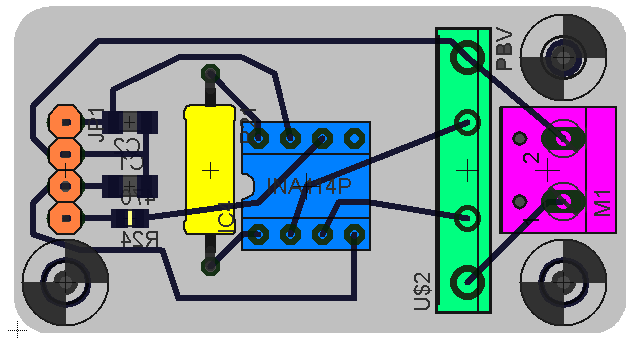
\includegraphics[width=75mm]{img/i2.png}
\caption{Die Platine zur Strommessung}\label{i2}
\end{figure}



\subsection{Das Shield}\thispagestyle{empty}
Unter einem Shield versteht man eine Platine die auf einem Arduino aufgesteckt werden kann, und benutzerspezifische Funktionalität beinhaltet. Im Falle des Messroboters befindet sich die 5V-Erzeugung, die -5V-Erzeugung, die SD-Karte und diverse Buchsen zum Anschluss der Messplatinen und des Sensorarray auf der Shield-Platine. 
Die SD-Karte benötigt eine 3.3V Versorgung, welcher der Arduino liefert. Dazu sind keine wieteren Bauteile nötig. 
Zusätzlich gibt es einen Pegelwandler, welcher die 5V-Level der digitalen Signale des Arduino auf 3.3V-Level für den SD-Karten.
In der Abbildung  \ref{shield} sind die verschieden Bauteile farbig markiert:
Klemmen zur Versorgung mit Akku-Spannung (rosa), Buchse zur Kommunikation mit der Sensor-Array Platine (violett). Eine 10-poligeBuchse zur Verbindung mit der Motortreiberplatine (violett). Insgesamt vier vierpolige Stecker (rosa) für verschiedene Messplatinen, wovon nur drei in Gebrauch sind: für die Strommessung und die beiden Temperaturmessungen.

\begin{figure}[htbp]
\centering
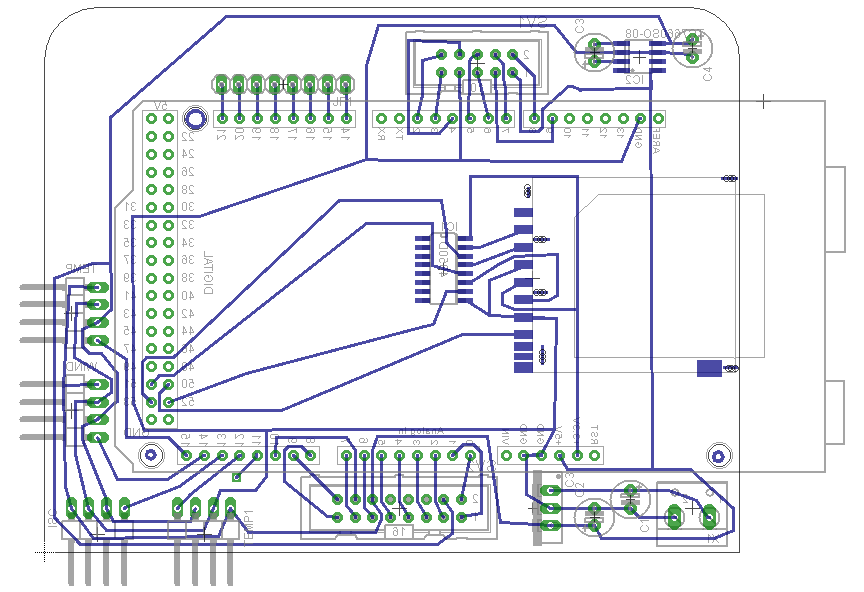
\includegraphics[width=125mm]{img/shield.png}
\caption{Die Shield-Platine.}\label{shield}
\end{figure}

\subsection{Temperaturmessung}\thispagestyle{empty}
Der Spannungsabfall an einem temperaturstabilen 100$\Omega$ Widerstand wird mit dem Spannungsabfall an einem PT100 verglichen. Durch beide Widerstände fließt ein Strom von 100$\mu$A. Als Stromquelle dient eine sehr präzise REF200-Stromquelle\cite{ref200}, welche zwei mal 100 Mikroampere $\pm$0.5$\%$ liefert. Abbildung \ref{tmess} zeigt den Schaltplan, Abbildung \ref{tmess2} zeigt das Platinenlayout. Zur besseren Idendifikation sind die Bauteile in beiden Abbildungen mit den gleichen Farben eingefärbt. 
Zum Platinenlayout: Links, der 4-pinige Stecker dient zur Stromversorgung (+5V, GND, -5V) und dem Abgriff des analogen Messsignales. Dimensionierung des Verstärkungswiderstandes: ...
Warum Präzisionswiderstände? Weil temperaturstabiler als herkömmliche Widerstände. 
Warum zwei Widerstände zum Einstellen der Verstärkung des Instrumentenverstärkers? Weil es keinen Präzesionswiderstand gab der in etwa dem berechneten Wert entsprach. Daher wurden zwei 51,1$ßOmega$ Widerstand parallel geschaltet, das entspricht einen 25,55$ßOmega$ Widerstand.


Was würde man heute anders machen? Der Temperaturbereich ist genauer bekannt. Damit könnte der Messbereich des ADC besser ausgenutzt werden. Nachher ist man immer klüger! Siehe Kapitel Kalibrierung. Erst dort wurde der maximal mögliche ADC- und Widerstandswert ermittelt, weil der Instrumentenverstärker nicht bis 5V aussteuern kann, sondern nur bis etwa 4,2V, bzw. einem ADC-Wert von etwa 850. Daher sollte der maximale Messwert wesentlich kleiner sein, damit Unklarheiten, ob die Begrenzung schon erreicht ist, vermieden werden. 


\begin{figure}[htbp]
\centering
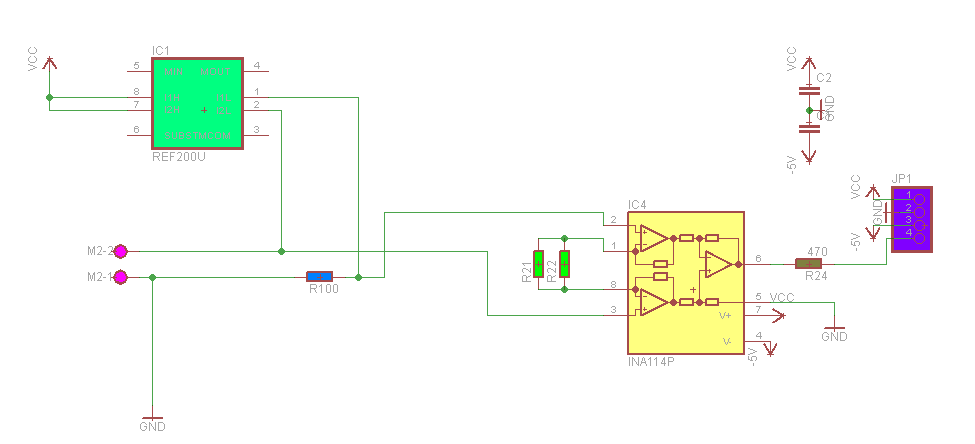
\includegraphics[width=125mm]{img/tmess.png}
\caption{Schaltung der Temperaturmessung}\label{tmess}
\end{figure}

\begin{figure}[htbp]
\centering
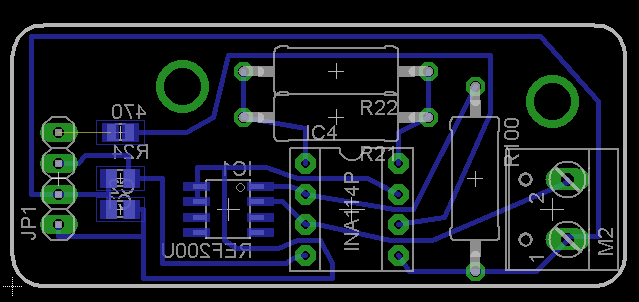
\includegraphics[width=100mm]{img/tmess2.png}
\caption{Layout der Temperarurmessung}\label{tmess2}
\end{figure}






\section{Softwareentwicklung}\thispagestyle{empty}
Dieser Abschnitt beschreibt die Entwicklung des Softwareteils. Es wird kurz auf die Entwicklungsumgebung eingegangen. Dann folgt die Auswertung der optischen Sensoren. Schließlich wird die Programmstruktur erklärt. Der gesamte Code ist im Anhang gelistet.

\subsection{Entwicklungsumgebung}\thispagestyle{empty}
Der Mikrocontroller auf den Arduino Board wird mit der Arduino Programmiersprache, welche auf Wiring basiert und sehr C-artig ist, in der Arduino Entwicklungsumgebung (siehe Abbildung \ref{ardu2}, welche auf Processing basiert, programmiert. Die Entwicklungsumgebung ist auf das notwendigste beschränkt. Die vielen Beipsielprogramme erlauben einen raschen Einstieg.
Ein Arduino Programm besteht aus zwei Teilen: Einer Setup-Routine die einmal zu Programmstart durchlaufen wird und einer Endlosschleife. In der Schleife wird das eigentlich Programm abgearbeitet. 

\begin{figure}[htbp]
\centering
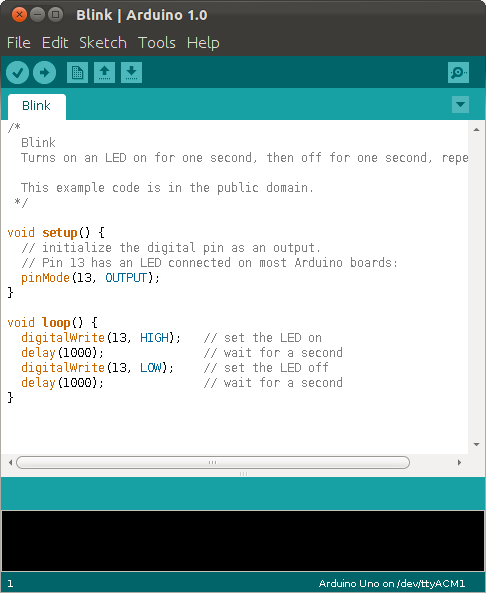
\includegraphics[width=100mm]{img/Arduino.png}
\caption{Die Arduino Entwicklungsumgebung}\label{ardu2}
\end{figure}

\subsection{Auswertung der optischen Sensoren}\thispagestyle{empty}
Um den Einfluss des Streulichtes der starken Einstrahlung im Sonnensimulator auf die Optoreflektoren CNY70 zu vermeiden, wurde eine differentielle Messmethode angewandt. Die Messwerte bei ausgeschalteter Infrarot-Leuchtdioden werden von den Messwerten mit eingeschalteter Leuchtdioden abgezogen.
Das wird für alle neun Optoreflektoren des Sensorarray, sowie den Stopsensor, gemacht.
Mit den korrigierten Werten der einzelnen optischen Sensoren wird die Lage der Linie relativ zum Mittelpunktes des Arrays bestimmt. 

Die Höhe des Messwertes  der optischen Sensoren ist abhängig von der Helligkeit des Untergrundes. Unter der Annahme dass sich eine gerade Linie unter dem Senorarray befindet funktioniert folgende Formel:
\begin{align*}
  x_1 &= \frac{C-A}{2A-4B+2C} \\
  \\
  x_2 &=  \frac{F-D}{2D-4E+2F} \\
  \\
  x_3 &=  \frac{I-G}{2G-4H+2I} \\
  \\
  d &=  \frac{x_1+x_2+x_3}{3} \\
  \\
  k &=  \frac{x_1-x_3}{2}
\end{align*}
Dabei ist es egal, ob es sich um eine helle Linie auf dunklen Untergrund, oder eine dunkle Linie auf hellem Untergrund handelt. Bei andere Teilen des Algorithmus ist das aber nicht egal. Daher funktioniert der Roboter nur mit heller Linie auf dunklen Untergrund.  Abbildung 

\begin{figure}
\centering
    \subfigure[Versatz]{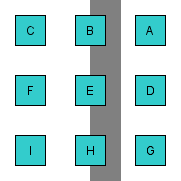
\includegraphics[width=50mm]{img/array5.png}}
    \subfigure[Verdrehung]{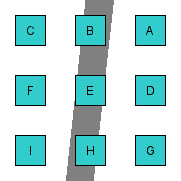
\includegraphics[width=50mm]{img/array6.png}}
\caption{Die mögliche Abweichungen der Linie von der Idealposition}
\label{abw}
\end{figure} 

Abbildung \ref{abw} zeigt die Anordnung des Sensorarrays, die einzelnen Sensoren sind mit A bis I bezeichnet. Mögliche Abweichungen der Linie von der Idealposition sind, auf der linken Seite, der zeitliche Versatz auf der rechten Seite, zu sehen.

\subsection{Auswertung der Temperatur- und Strommesswerte}\thispagestyle{empty}
Aufgrund von Rauschen der ADC-Werte, wurden alle Messwerte über 500 Einzelmessungen gemittelt. Die Quelle des Rauschens wurde nicht ermittelt. Der notwendige Messzeit dafür beträgt unter einer halben Sekunde. Ohne Mittelung des Messwerte schwankten die Messungen $\pm$5 Werte des ADC, das sind $\pm$0,5$\%$ bei maximalen Ausnützung bzw. $\pm$1$\%$ bei halber Ausnützung des ADC Wertebereichs.
 
\subsection{Programmablauf}\thispagestyle{empty}

Das Steuerprogramm ist als Zustandsautomat konzipiert (siehe Abbildung \ref{abl}):
\begin{itemize}
\item Zustand s (Start): zu Programmstart, nach 60 Sekunden Wechsel in den Zustand v. Diese Zeitspanne dient zum schließen des Messeinschubes des Sonnensimulators nach dem Einschalten des Roboters.
\item Zustand v: Vorwärtsfahren inklusive Regelung, Wechsel durch erkannte Ecke in den Zustand a, bzw. durch erkannten Messpunkt Wechsel in den Zustand m.
\item Zustand z: Rückwärtsfahren inklusive Regelung, Wechsel durch erkannte Ecke in den Zustand c, bzw. durch erkannten Messpunkt Wechsel in den Zustand m.
\item Zustand m: Messpunkt, nach Abschluss der Messung wird der bisherige Messmodus fortgesetzt.
\item Zustand r: Rechtsfahren mit Regelung, nach erkannter Ecke Wechsel in den Zustand b.
\item Zustand l: Ebenfalls Rechtsfahren mit Regelung, nach erkannter Ecke Wechsel in den Zustand d.
\item Zustand a: Um die Ecke des Typ 1 fahren, danach Wechsel in den Zustand r. 
\item Zustand b: Um die Ecke des Typ 2 fahren, danach Wechsel in den Zustand x.
\item Zustand c: Um die Ecke des Typ 1 fahren, danach Wechsel in den Zustand l. 
\item Zustand d: Um die Ecke des Typ 2 fahren, danach Wechsel in den Zustand p.
\item Zustand p, x: Ausrichten, danach Wechsel zu q bzw. y.
\item Zustand q, y: Ausrichten, danach Wechsel zu v bzw. z.
\end{itemize}

Ein paar Worte zur Regelung der Geradeausfahrt: 
Es wird versucht sowohl die seitliche Verschiebung d als auch die Verdrehung zu minimieren. Wenn beide Werte innerhalb gewisser Toleranzen sind, fährt der Roboter geradeaus. Die Schranken der Regelung sind in Abbildung \ref{schr} zu sehen. 

Und nun zur Regelung der Seitwärtsfahrt. Wieder wird versucht die Abweichung in Verschiebung, diesmal in vor- und zurück-Richtung, und der Verdrehung zu minimieren.  Allerdings hat das Seitwätsfahren eine andere Dynamik als das Geradeausfahren. Die Geradeausfahrt eines Mecanum-Fahrzeuges ist vergleichbar mit der eines konventionellen Fahrzeuges. 
Bei der Seitwärtsfahrt wurde eine verbesserte Regelung angewandt, statt zwei Dreipunktreglern, wurde zwei P-Regler verwendet. Dabei wird zur Fahrt nach Rechts eine Vor/Zurück-Fahrt und eine Drehung überlagert. Somit gibt es keine ruckartigen Übergänge von einer Bewegung zur nächsten.

\begin{verbatim}
  vz = int(800*d2);
  turn = int(2400*k2);

  M1(127 + vz + turn);
  M2(-127 + vz - turn);
  M3(-127 + vz + turn);
  M4(127 + vz - turn); 
\end{verbatim}

Da die Linie für das Rechtsfahren nicht in einer Ecke endet, sondern einfach endet, kann die Regelung bis zum Ende verwendet werden. Somit entfällt ein Teil des um-die-Ecke-Fahrens. Die Faktoren des P-Regler (800, 2400) wurden durch umfangreiche Testfahrten ermittelt.

Es gibt zwei Arten von Ecken. Einmal die Ecke des Typs 1, welche eine wirkliche Ecke darstellen. Und dann die Ecke des Typs 2, welches ein Eck mit einer Lücke sind.
Die beiden unterschiedlichen Arten von Ecken wurden begründet durch die unterschiedlichen Fahreigenschaften/ Fahrdynamik beim Geradeausfahren und dem Seitwärtsfahren. Deshalb gibt es beim Seitwärtsfahren auch den weiterentwickelten Regelungsalgorithmus, der sich dann aber als sehr kompakt herausgestellt hat.

\begin{figure}[htbp]
\centering
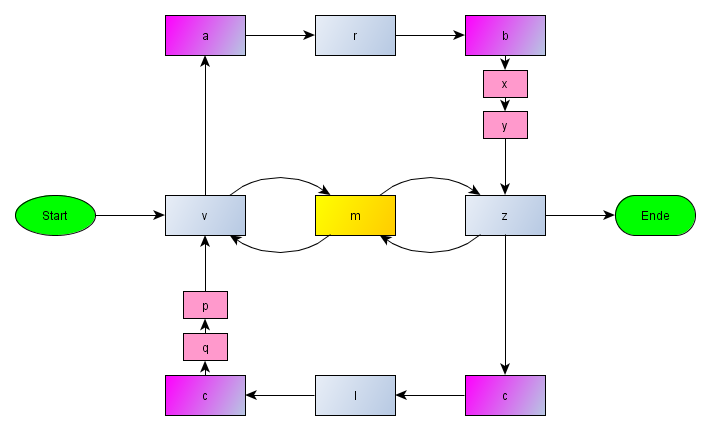
\includegraphics[width=150mm]{img/ablauf2.png}
\caption{Der Programmablauf}\label{abl}
\end{figure}

\begin{figure}[htbp]
\centering
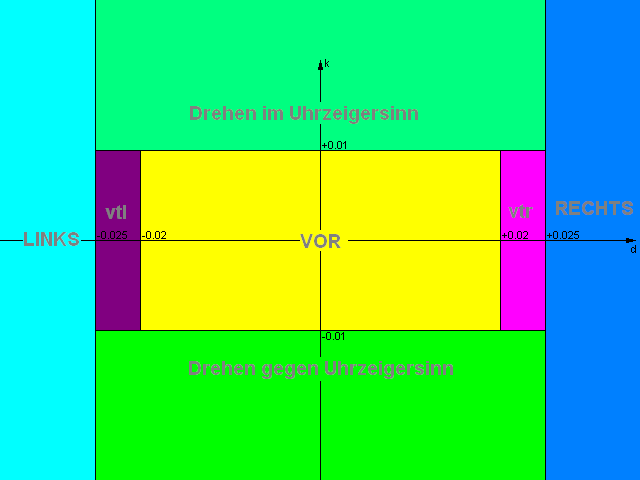
\includegraphics[width=80mm]{img/schranken.png}
\caption{Schranken der Regelung}\label{schr}
\end{figure}

\begin{figure}[htbp]
\centering
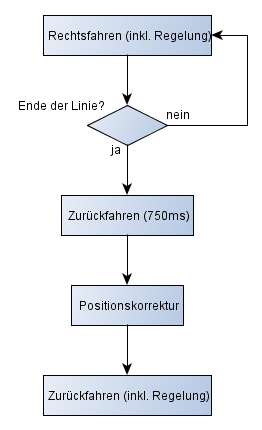
\includegraphics[width=50mm]{img/ecke2.png}
\caption{Ums Eck fahren}\label{eck}
\end{figure}


\chapter{Kalibration}\thispagestyle{empty}

Dieses Kapitel beschreibt die Kalibrierung der Messsensoren. Es gibt drei Messplatinen, eine für die Messung des Kurzschlussstromes der Messzelle, und zwei identisch aufgebaute Messplatinen zur Messung der Zelltemperatur beziehungsweise der Umgebungstemperatur. Die Strom-Messplatine wandelt den Kurzschlussstrom der Messzelle in eine Spannung um, die in einem für den ADC des Arduino auswertbaren Bereich (0 bis 5 Volt) ist. Die beiden Messschaltungen zur Temperaturmessung wandeln die Größe der temperaturabhängigen Messwiderstände, jeweils ein Pt-100, in eine Spannung um.
Die ADC-Messwerte wurden über die USB-Schnittstelle des Roboters ausgelesen. Dafür benötigt der Roboter ein einfaches Kalibrierprogramm.



\section{Temperatursensoren}\thispagestyle{empty}
Die Temperatur der Messzelle wird mit einem von unten aufgeklebten flächigen Folienmesswiderstand gemessen. 
Ein zweiter Pt100, in kompakter Dünnschichtbauweise ausgeführt, misst die Temperatur der Umgebung. Beide Messskreise sind identisch aufgebaut, dennoch führen Bauteiltoleranzen zu leicht unterschiedlichen Verstärkungen.
Für die Kaltbration der Temperaturmesselektronik wurden die Pt-100 Widerstände durch einen hoch genaues, einstellbares und kalibriertes Messnormal ersetzt. Der Widerstand wurde im Bereich von 100 bis 122 	$\Omega$  in 1 $\Omega$  Schritten verändert, was einer Temperatur von 0 bis 55 $^{\circ}$C entspricht. Die ADC-Werte wurden über die USB-Schnittstelle des Arduino ausgelesen. Es zeigte sich, dass die beiden Schaltungen leicht unterschiedliche Verstärkungen haben. Daher mussten jede Temperaturmessschaltung separat kalibriert werden.

\begin{table}[htbp]
\centering
\begin{tabular}{ | c | c | }\hline
{\bf R / $\Omega$ } & {\bf ADC Wert}\\ \hline
\hline
101 & 12\\ \hline
102 & 53\\ \hline
103 & 93\\ \hline
104 & 133\\ \hline
105 & 173\\ \hline
106 & 212\\ \hline
107 & 253\\ \hline
108 & 293\\ \hline
109 & 332\\ \hline
110 & 374\\ \hline
111 & 412\\ \hline
112 & 454\\ \hline
113 & 493\\ \hline
114 & 533\\ \hline
115 & 573\\ \hline
116 & 613\\ \hline
117 & 653\\ \hline
118 & 694\\ \hline
119 & 734\\ \hline
120 & 775\\ \hline
121 & 815\\ \hline
122 & 857\\ \hline
\end{tabular}
\caption{Die Messwerte der Kalibrierung Messschaltung A}\label{TabA}
\end{table}

Obwohl der 10-Bit ADC des Arduino einen Maximalwert von 1023 hat, ist bedingt durch den Einsatz des Instrumentenverstärkers INA114, der maximale ADC-Wert bei 857, was einer Spannung von 4,18V entspricht.  


\begin{figure}[htbp]
\centering
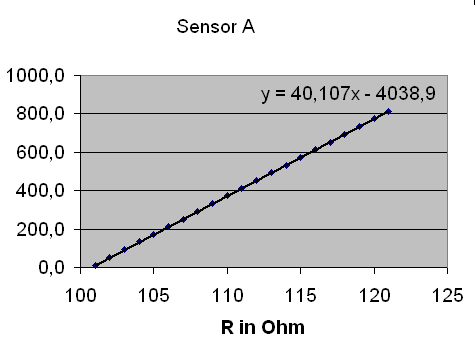
\includegraphics[width=100mm]{img/messa.png}
\caption{Ausgleichsgerade Temperaturmessung A}\label{messa}
\end{figure}

\begin{table}[htbp]
\centering
\begin{tabular}{ | c | c | }\hline
{\bf R / $\Omega$ } & {\bf ADC Wert}\\ \hline
\hline
100 & 0\\ \hline
101 & 20\\ \hline
102 & 60\\ \hline
103 & 99\\ \hline
104 & 139\\ \hline
105 & 179\\ \hline
106 & 219\\ \hline
107 & 259\\ \hline
108 & 299\\ \hline
109 & 339\\ \hline
110 & 379\\ \hline
111 & 420\\ \hline
112 & 460\\ \hline
113 & 499\\ \hline
114 & 539\\ \hline
115 & 579\\ \hline
116 & 619\\ \hline
117 & 659\\ \hline
118 & 700\\ \hline
119 & 740\\ \hline
120 & 780\\ \hline
121 & 820\\ \hline
122 & 857\\ \hline
\end{tabular}
\caption{Die Messwerte der Kalibrierung Messschaltung B}\label{TabB}
\end{table}

\begin{figure}[htbp]
\centering
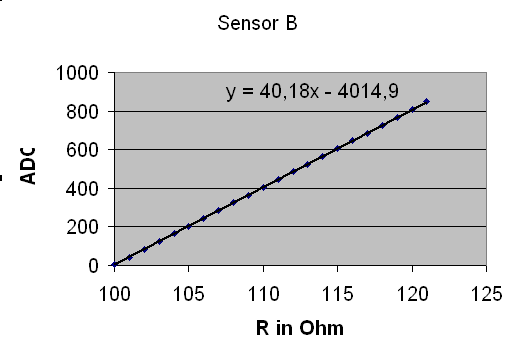
\includegraphics[width=100mm]{img/messb.png}
\caption{Ausgleichsgerade Temperaturmessung B}\label{messb}
\end{figure}

Die mit Excel gewonnen Gleichungen der Ausgleichsgerade für Messschaltung A (siehe Abbildung ~\ref{messa}) und B (siehe Abbildung ~\ref{messa}) werden verwendet um aus den ADC-Werten die dazugehörigen Widerstandswerte zu berechnen. 

  \begin{equation}
     R_A(ADC) = \frac{ADC_A + 4039,9}{40,107}
  \end{equation}
  
    \begin{equation}
     R_B(ADC) = \frac{ADC_B + 4023,6}{40,027}
  \end{equation}


\section{Messzelle}\thispagestyle{empty}


Der Kurzschlussstrom der Messzelle wurde im Flasher (siehe Abbildung~\ref{zelleflasher}) über einen weiten Temperaturbereich gemessen (siehe Abbildung~\ref{tempkoef}). Es wurde mit der Berger Messlast \cite{berger} gemessen. Bei der Messung wurden die Leitungswiderstände der Messkabel minimiert, indem Kabel mit hohem Querschnitt (6mm$^2$) verwendet wurden, und die Kabel möglichst kurz gehalten wurden (<1,5m).
 
\begin{figure}[htbp]
\centering
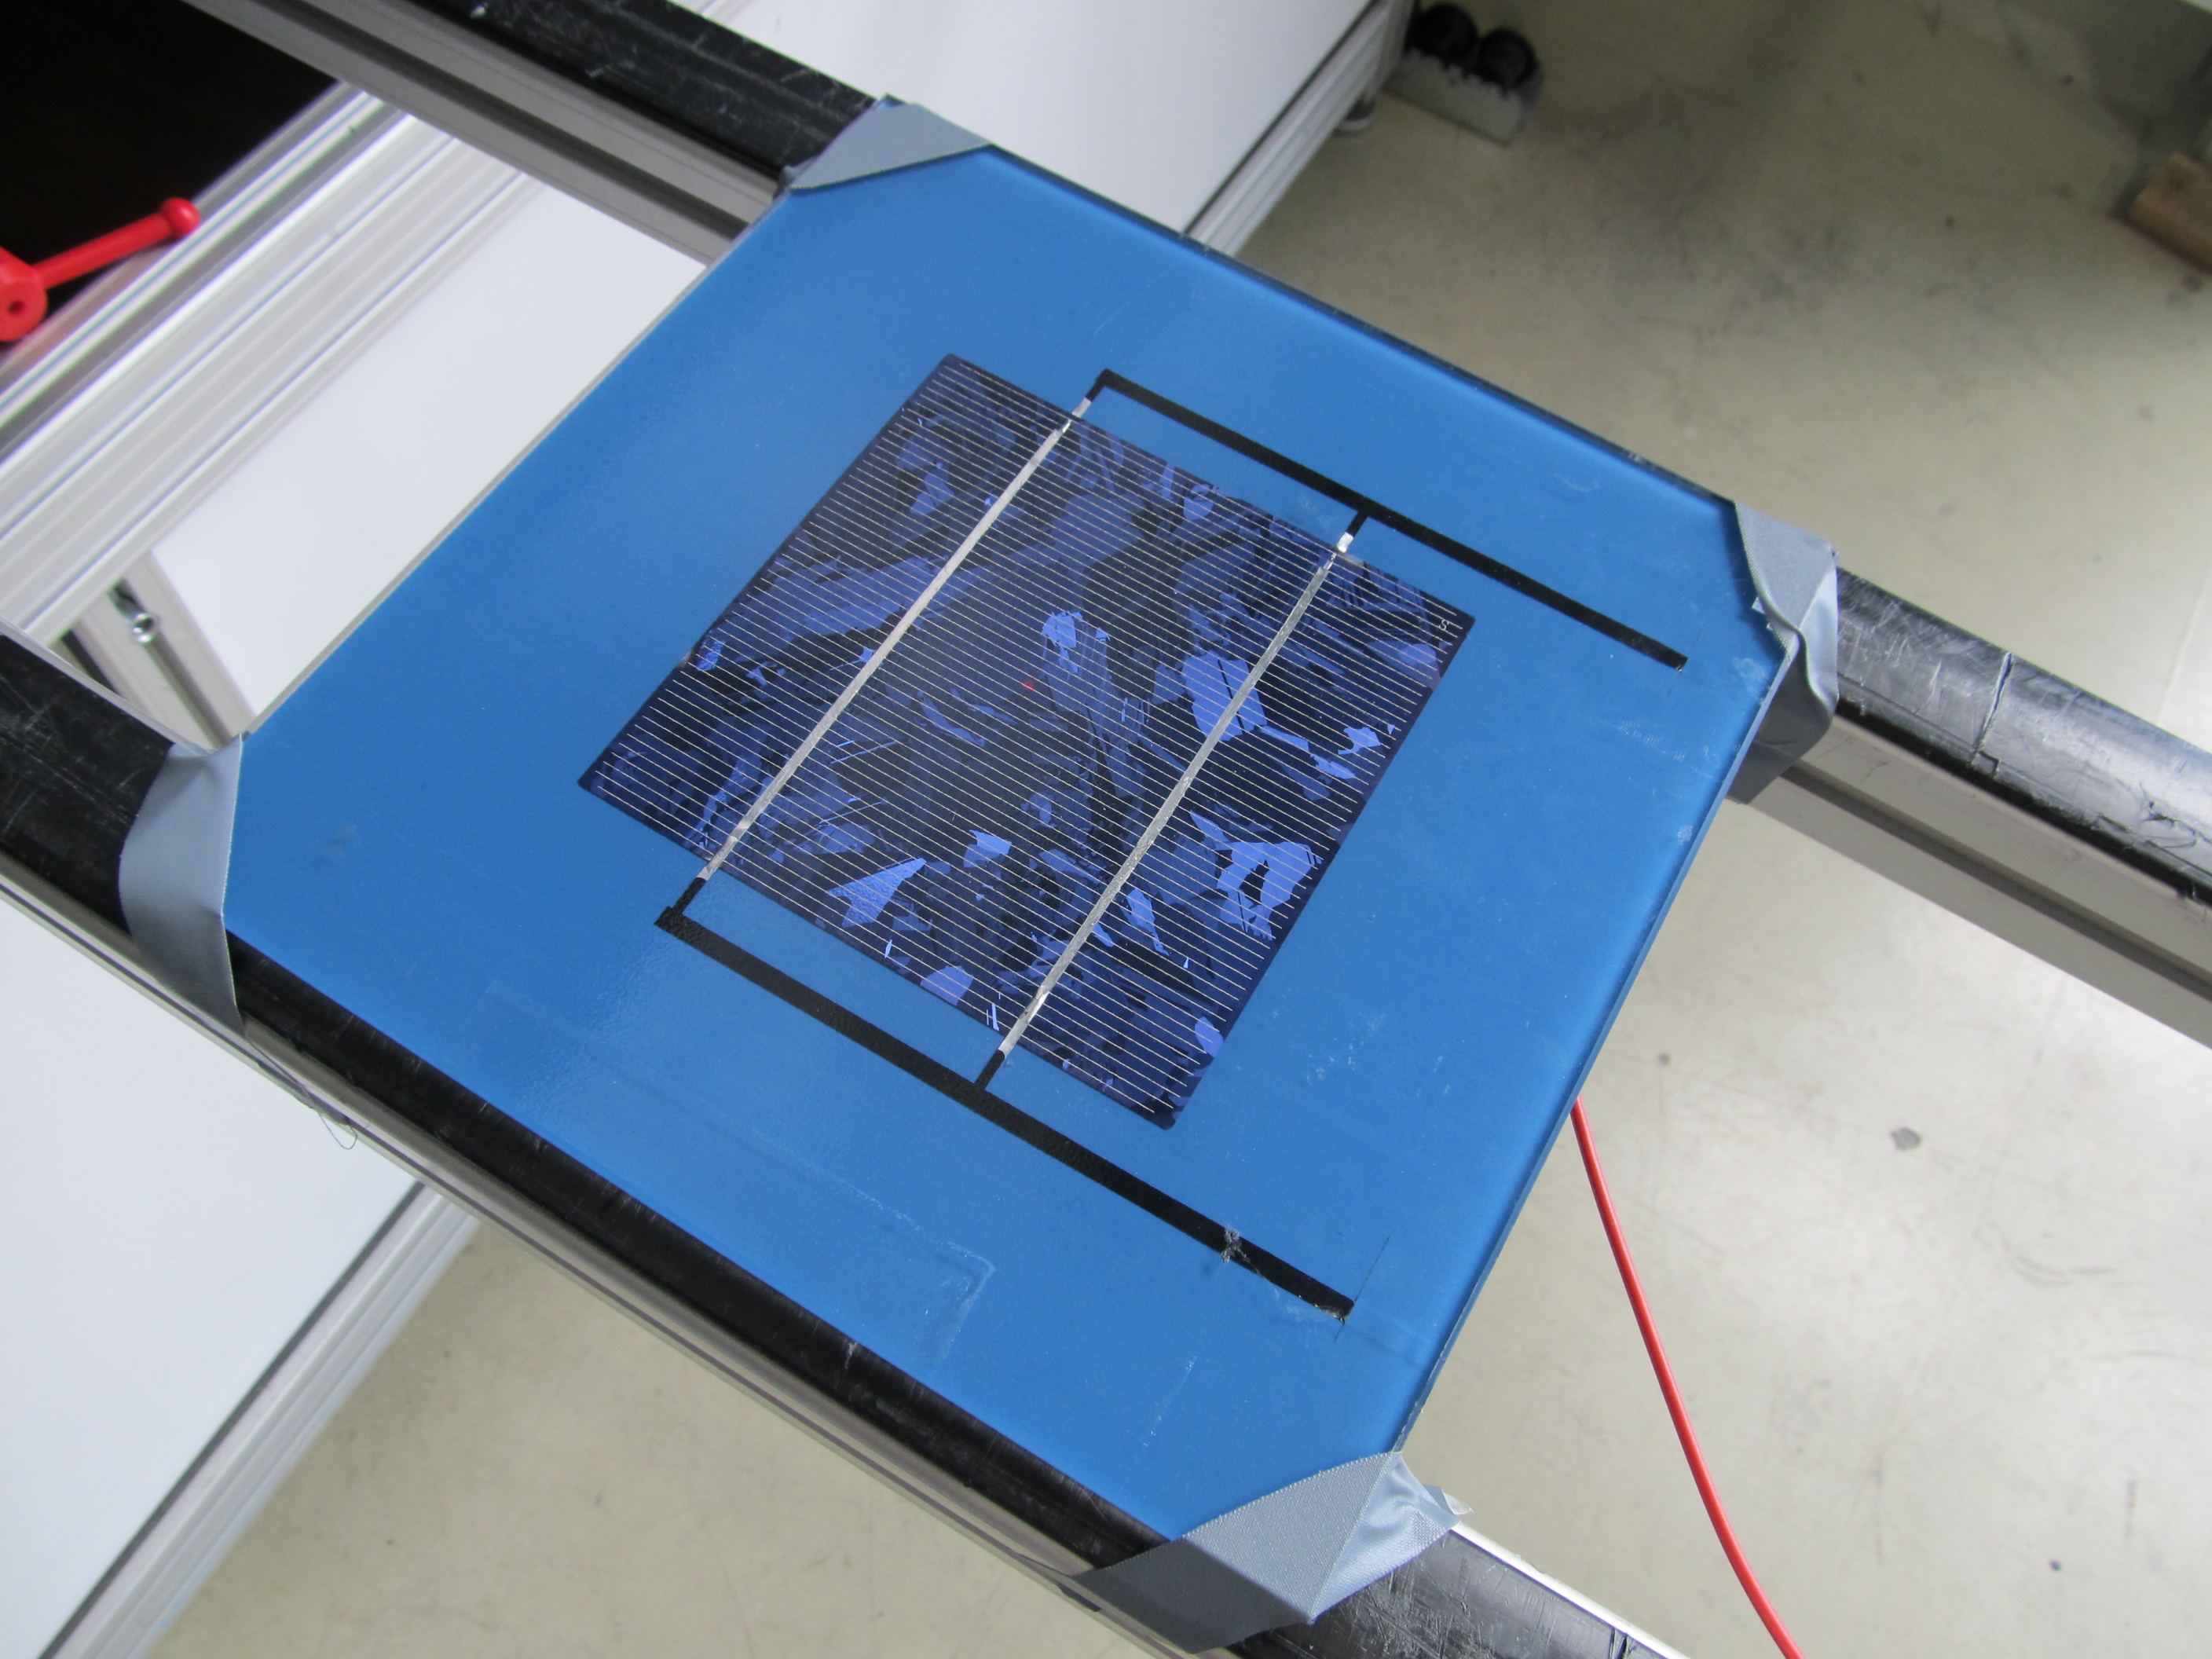
\includegraphics[width=75mm]{img/zelle.jpg}
\caption{Ein Photo der Messzelle}\label{zelleflasher}
\end{figure}

\begin{figure}[htbp]
\centering
\includegraphics[width=150mm]{img/Isc.png}
\caption{Abhängigkeit des Kurzschlussstromes von der Temperatur}\label{tempkoef}
\end{figure}

  \begin{equation}
     I(T) = 4,9529+0.0024 \ast T
  \end{equation}
  
    \begin{equation}
     I(T) = 4,9529 \ast ( 1 + 0,00048 \ast T)
  \end{equation}

\section{Strommessung}\thispagestyle{empty}

Der Messroboter wurde für die Kalibrierung der Strommessung in eine Klimazelle platziert.  Die Temperatur der Klimazelle wurde im Bereich von 8 bis 35 $^{\circ}$C variiert. Durch den Messwiderstand der Strommessung wurde ein Strom im Bereich von 3 bis 8 A geschickt.  

\begin{table}[htbp]
\centering
\begin{tabular}{|l|l|l|}
\hline
T/$^{\circ}$C & I/mA & ADC Wert \\ 
\hline
\hline

\multirow{3}{*}{24,4} & 3997 & 472 \\
 & 6001 & 712 \\
 & 8002 & 854 \\ \hline
\multirow{3}{*}{35,3} & 3999 & 473 \\
 & 6001 & 712 \\
 & 7999 & 859 \\ \hline
\multirow{3}{*}{35,3} & 3999 & 472 \\
 & 6001 & 710 \\
 & 8001 & 852 \\ \hline
\multirow{5}{*}{16,4} & 2004 & 234 \\
 & 3005 & 353 \\
 & 4003 & 473 \\
 & 5003 & 591 \\
 & 6005 & 711 \\ \hline
\multirow{5}{*}{8} & 1993 & 233 \\
 & 2995 & 352 \\
 & 4001 & 472 \\
 & 5000 & 590 \\
 & 6005 & 710 \\ \hline
\end{tabular}
\caption{Kalibrierung Strommessung}\label{TabS}
\end{table}

\begin{figure}[htbp]
\centering
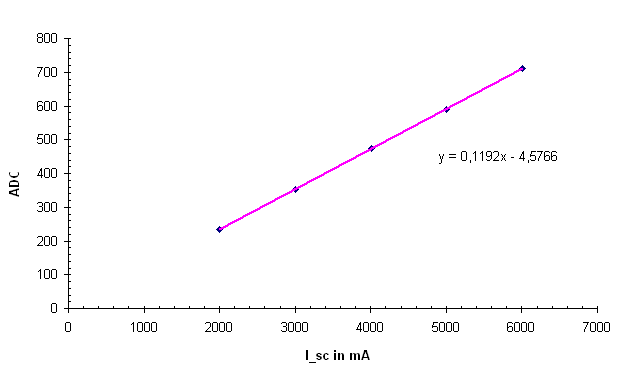
\includegraphics[width=150mm]{img/16grad.png}
\caption{Lineraer Zusammenhang zwischen Strom und dem ADC-Wert}\label{ical}
\end{figure}

\begin{equation}
     I(ADC) = \frac{ADC + 4,5766} {119,2} 
\end{equation}
  


\section{Thermische Stabilität der Temperaturmessung}\thispagestyle{empty}
Zur Bestimmung der Temperaturstabilität wurde der gesamte Roboter in ein Klimakammer gestellt. Der Pt100 wurde durch einen temperaturstabilen 110$\Omega$ simuliert.
Es gab zwei Durchgänge dieses Versuches.
Bei der ersten Messung zeigte sich, dass eine der beiden Messplatinen nicht temperaturstabil war. Durch das Tauschen der Ref200 Stromquelle dieser Platine konnte das Problem gelöst werden.

\begin{table}[htbp]
\centering
\begin{tabular}{ | c | c | c |}\hline
{\bf T / $^{\circ}$C} & {\bf ADC Platine A} & {\bf ADC Platine B}\\ \hline
\hline
11,7 & 368 & 407\\ \hline
13,0 & 368 & 406\\ \hline
13,7 & 368 & 406\\ \hline
14,5 & 368 & 405\\ \hline
15,5 & 368 & 405\\ \hline
16,6 & 368 & 405\\ \hline
17,5 & 368 & 404\\ \hline
23,5 & 368 & 403\\ \hline
27,5 & 368 & 402\\ \hline
\end{tabular}
\caption{Temeraturabhängigkeit der Temperaturmessung}\label{TabT1}
\end{table}

\begin{table}[htbp]
\centering
\begin{tabular}{ | c | c | c |}\hline
{\bf T in $^{\circ}$C} & {\bf ADC Platine A} & {\bf ADC Platine B}\\ \hline
\hline
30,7 & 368 & 380\\ \hline
20,1 & 368 & 379\\ \hline
9,2 & 368 & 378\\ \hline
\end{tabular}
\caption{Temeraturabhängigkeit der Temperaturmessung}\label{TabT2}
\end{table}

Durch den Austausch der Referenzstromquelle der Platine B hat sich auch der ADC-Wert gegenüber der ersten Messung geändert. Die Kalibrierwerte der Platine B \ref{TabB} sind nach diesem Austausch aufgenommen worden.
Da die Platine A temperaturstabiler als die Platine B ist, wurde Platine A zur Messung der Zelltemperatur ausgewählt, die Platine B wurde für die Messung der Umgebungstemperatur verwendet. 

\chapter{Messung}\thispagestyle{empty}

Diese Kapitel beschreibt die Messvorbereitung, den Messaufbau, die eigentliche Messung und die Auswertung der Messdaten. Um was geht es? Um die Messung. Zur Messung gehört der Messaufbau, der Messablauf und die Auswertung der Messung. Weiters werden Messungen bei verschiedenen Einstellungen diskutiert. 

\section{Messaufbau}\thispagestyle{empty}
Dieser Abschnitt behandelt den Messaufbau. Die Messung der Bestrahlungsstärkeverteilung findet im Sonnensimulator statt. Zuerst muss eine Messebene geschaffen werden. Die, im normalen Messalltag vermessenen, Module liegen auf verschiebbaren Metallschienen auf. Damit der Roboter fahren kann, braucht er eine ebene Fläche. Diese Fläche ist aus logistischen Gründen aus drei einzelnen Holzplatten gebildet, was einige zusätzliche Probleme bereitet hat. Auf der Oberseite der Platten befindet sich die Messpunkte und eine Führungslinie, welcher der Roboter folgt. Zur Messung wird der Roboter an das linke Ende der Linie gestellt, er fährt nach dem Einschalten selbständig das Messprogramm ab.

\begin{figure}[htbp]
\centering
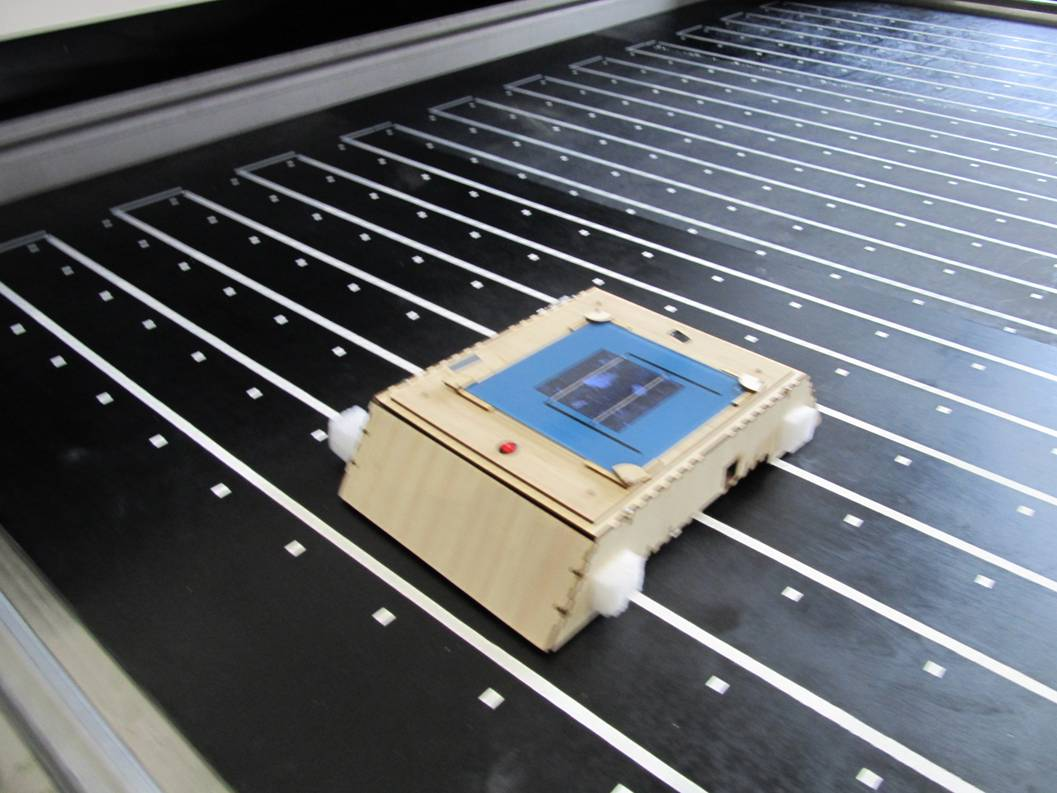
\includegraphics[width=100mm]{img/robofahrt.jpg}
\caption{Eine Fahrt des Roboters auf der Messbahn}\label{robofahrt}
\end{figure}

  \subsection{Platten}\thispagestyle{empty}
Drei Holzplatten bilden die Messebene für den Roboter. Eine große Platte wäre eine bessere Alternative gewesen, aber aus logistischen Gründen ist die Messebene auf drei Platten aufgeteilt. Weil für die drei Platten leichter ein Platz zum Aufbewahren gefunden werden kann. Die 250 mal 125 Zentimeter großen und 18 Millimeter dicken Holzplattenlatte sind gerade noch hantierbar. 
Die Platten sind schwarz, damit sie einen möglichst geringen Reflexionskoeffizienten haben. Um einen großen Unterschied im Reflexionskoeffizienten zu haben, ist die Messbahn weiß gehalten. Sowohl der schwarze Untergrund als auch die weiße Bahn ist mit Kunstharzfarbe ausgeführt. Beim Hantieren mit den Platten können kleine Beschädigungen der Messbahn entstehen. Da diese Beschädigungen  den Messablauf stören können, ist es ratsam vor der Messung die Bahn mit einem weißen Klebeband (Isolierband) auszubessern.
Die Platten müssen eng aneinander anliegen, damit der Roboter von einer Platte zur anderen fahren kann. Damit keine zu groß Stufe wegen unterschiedlicher Duschbiegung der Platten entsteht ist auf der Rückseite der Holzplatten Aluminiumbleche befestigt, auf einer Seite angeschraubt, die danebenliegende Platte liegt darauf.
Da die Breite aller 3 Platten geringer ist als die Breite der Lade des Sonnensimulators, werden, damit die Messungen zu verschiedenen Zeitpunkten verglichen werden können, die Platten so weit wie möglich nach rechts geschoben. Am Rand liegen die Platten auf Aluschienen auf.
Die Messpunkte liegen im Raster von 15 Zentimeter. Die Führungslinie 25,4 Millimeter daneben, gemessen vom Zentrum des Messpunktes zur Mitte der Linie. Die Messpunkte sind kleine Quadrate der Seitenlänge von 14 bis 15 Millimeter. Die Messbahn ist ebenfalls 14 bis 15 Millimeter breit. Die Position der Messpunkte ist auf etwa ein bis zwei Millimeter genau.
Die Messpunkte liegen im Abstand von 15 cm, damit ist auch der Abstand zwischen den Messbahnen 15 cm, der Roboter muss nur 15 cm seitwärts fahren. Die Übergänge der Messbahn von einer Platte zur nächsten sind mit weißem Isolierband  der Breite 14 Millimeter zu überbrücken. Beschädigung der Messbahn, welche durch unsanftes Handling der Platten entstehen können, sind ebenfalls mit weißem Isolierband zu Überkleben.
Die Messebene wird aus 3 Holzplatten gebildet, diese sind auf der Oberseite schwarz gefärbt und mit einer weißen mäanderförmigen Spur versehen. Die Platten hängen durch, dadurch ist die Messebene nicht eben. Schlimmer ist der nicht gleiche Durchhang verschiedener Platten. So kommt es zu einem Höhenunterschied zwischen den Platten. Um diese Stufen zu verringern wurde auf der Unterseite der Platten mit dem geringeren Durchhang eine kleine Aluplatte befestigt um eine Auflage für die andere Platte zu schaffen. Eine zu große Stufe behindert den Roboter beim Fahren. Weil an der Stufe nicht alle Haltepunkte zuverlässig erkannt werden können.


\begin{figure}[htbp]
\centering
\includegraphics[width=125mm]{img/messbahn1.png}
\caption[Messbahn auf den Platten]{Messbahn auf den Platten}\label{bahn}
\end{figure}






\subsection{Ablauf}\thispagestyle{empty}
Vor der Messung ist der Akku des Roboters voll zu laden. Der roboter ist auf mechanische Beschädigung zu Untersuchen, eventuell ist ein Rad locker, dann lässt es sich entlang der Achse verschieben.
Zuallererst sind die Platten auf Beschädigung zu untersuchen. Beschädigungen der Messbahn sind mit einem weißen Isolierband zu überkleben. Beschädigungen des Holzes direkt neben der Messbahn sind mit schawrzer Farbe auszubessern. Stellen, die der Sensor nicht sehen kann, sind egal.
Die Platten sind in den Einschub des Sonnensimulators zu legen. Das ist ein Puzzle und nicht schwer. Beginnend rechts. Die Übergänge der Messbahn von einer Platte zur nächsten sind mit weißem Isolierband  der Breite 14mm zu überbrücken. Beschädigung der Messbahn, welche durch unsanftes Handling der Platten entstehen können, sind ebenfalls mit weißem Isolierband zu Überkleben.



Roboter wird auf das linke vordere Ende der Messbahn gestellt. Der Roboter muss dabei auf der Messbahn stehen. Kleinere Abweichungen der Idealposition werden beim losfahren korrigiert. 
Vor der eigentlichen Messfahrt ist eine Testfahrt mit geöffneter Lade des Sonnensimulators zu empfehlen. Besonders die Übergänge von einer Platte zur nächsten können Probleme schaffen.
Nach der bestandenen Testfahrt wird der Sonnensimulator eingeschaltet. Bis zur Messung sind 20 bis 30 Minuten zu warten, bis die Temperaturen im Simulator stabil sind. Der Roboter kann während dieser Zeit im Sonnensimulator stehen. Die Messzelle sollte allerdings abgeschattet werden, damit diese sich nicht aufheizt. 
Zum Starten wird der Schalter von 0 auf 1 umgelegt. Damit wird der Mikrocontroller mit Spannung versorgt. Das Programm startet. Nach einer Pause von 60 Sekunden, die zum Schließen des Sonnensimulators notwendig ist, fährt der Roboter los. Eine Messfahrt dauert etwa 13 Minuten. Nach Ablauf dieser Zeit wird der Roboter entnommen und die Daten der SD-Karte entnommen, oder der Roboter wird auf die Startposition gestellt um weitere Messfahrten durchzuführen.


\section{Auswertung}\thispagestyle{empty}


Die Messwerte werden auf SD-Karte als Textdatei gespeichert. Für jeden Messwert gibt es eine eigene Zeile. In jeder Zeile sind Messzeit in Millisekunden, der ADC-Wert für den Kurzschlussstrom, der ADC Wert für die Zelltemperatur, der ADC Wert für die Umgebungstemperatur, und jeweils einen Zählerwert für Messpunkt, Reihe und Spalte. Die einzelnen Werte sind durch einen Tabulator getrennt, damit ist die Datei in Excel und Matlab bearbeitbar.  

Die Tabelle \ref{TabSD} zeigt wie die Daten auf der SD-Karte gespeichert sind. Es sind nicht alle Werte für die Auswertung notwendig. Der Erste Wert ist die Zeit in Millisekunden, die seit dem Einschalten des Roboters vergangen ist. Die nächsten 3 Werte sind werte des Analogdigtalwandlers im Bereich von Null bis 1023, diese Werte werden ohne Umrechnung direkt auf die SD Karte gespeichert. Es sind 308 Messpunkte, 14 mal 22, es kann vorkommen, am Übergang von einer Platte zur anderen, dass ein Messpunkt ausgelassen wird. Das ist erkennbar wenn nicht 308 Messwerte im datalog-File sind. Um den Fehler leicht zu finden wurde Spalte und Reihe mit aufgezeichnet. Sind in einer Spalte nur 13 Messwerte, fehlt in dieser Spalte ein Wert. Anhand der mit aufgezeichneten Zeit kann der fehlende Messpunktes lokalisiert werden. Das geschieht nicht automatisch Der Messwert wird anhand der neben liegenden Werte geschätzt. Alternativ werden nur Messfahrten mit allen Punkten ausgewertet.
 
\begin{table}[htbp]
\centering
\begin{tabular}{ | c | c | c | c | c | c | c | } 
\hline
$\frac{t}{ms}$ & I$_{SC}$ & T$_{Zelle}$ & T$_{Umgebung}$ & Messpunkt & Messpunkt 2 & Messreihe \\
\hline
\hline
{165515} & {466} & {437} & {237} & {47} & {5} & {4} \\
\hline
{167523} & {479} & {437} & {235} & {48} & {6} & {4} \\
\hline
{169551} & {471} & {437} & {228} & {49} & {7} & {4} \\
\hline
\end{tabular}
\caption{Ein Ausschnitt der Messwertedatei}\label{TabSD}
\end{table}

Im Zuge der Auswertung wird ein eindimensionales Array von 308 Messwerten in ein zweidimensionales Array von 14 mal 22 Zahlen umgewandelt. Dazu wird der erste bis zum 14. Wert des eindimensionalen Arrays zur ersten Reihe des zweidimensionalen Arrays. Der 15. bis zum 28. Wert des eindimensionalen Arrays bilden die zweite Reihe des zweidimensionalen Arrays, allerdings in umgekehrter Reihenfolge. So bildet die Reihenfolge der Messwerte des zweidimensionalen Arrays die Messfahrt des Roboters ab.
\newline

\begin{equation}
\begin{pmatrix}
n_1 \\ . \\ . \\ . \\ n_{308} 
\end{pmatrix}
\Longrightarrow
\begin{pmatrix}
n_{1}  & . &.& .& n_{14} \\
n_{28} & .& .& . &n_{15}  \\
n_{29}  &. &.& .& n_{42}  \\
. &.& .& . & . \\
n_{295}  &.& .&.& n_{308} 
\end{pmatrix}
\end{equation}

Um die eindimensionale Datenwurst Datenwurst in ein zweidimesionales Array, das der realen Anordnung der Messpunkte entspricht, wird folgender Algorithmus verwendet:
\begin{verbatim}
j=1; k=1; l=1;

for(i=0:307)
    if(mod(i,28)>13) k = 28- mod(i,28);
    else k = mod(i,14)+1;
    end
    B(k,l)=A(i+1);
    if(mod(i+1,14)==0) l=l+1;
    end
end
\end{verbatim}

Beschreibung verbal: Es gibt 308 Messwerte. Die ersten 14 werden in die erste Reihe des Arrays gelegt. Die nächsten 14 in die zweite Reihe, aber in in absteigender Reihenfolge. Das heißt in die 14. Spalte der 2. Reihe wird der 15 Wert gelegt, also erste Reihe von links nach rechts, die zweite Reihe von rechts nach links, die dritte Reihe wieder von links nach rechts, usw.







Der ADC Wert des Kurschlussstromes wird in Ampere umgerechnet. Verwendet wird dazu die in im Abschnitt Kalibrierung gewonnene Formel.

\begin{figure}[htbp]
\centering
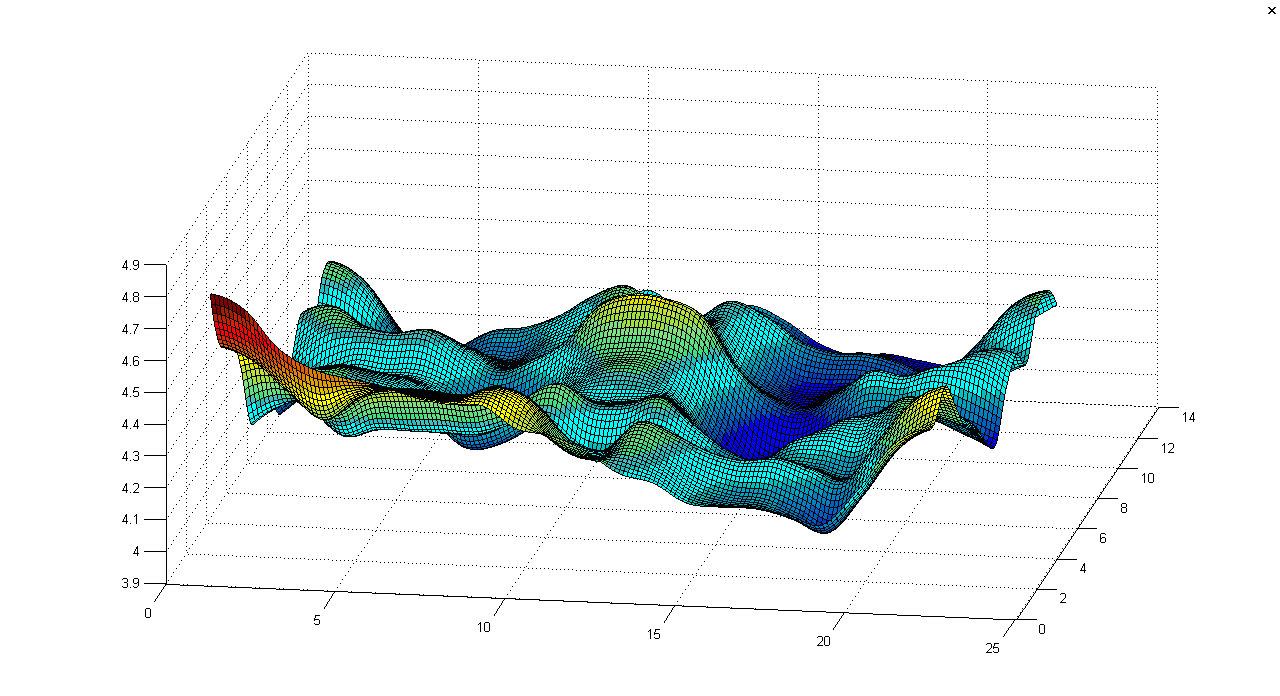
\includegraphics[width=150mm]{img/hugel.png}
\caption[Kurzschlusstromes in Ampere]{Verteilung des Kurzschlusstromes in Ampere abhängig von der Position}\label{hugel}
\end{figure}



\begin{figure}[htbp]
\centering
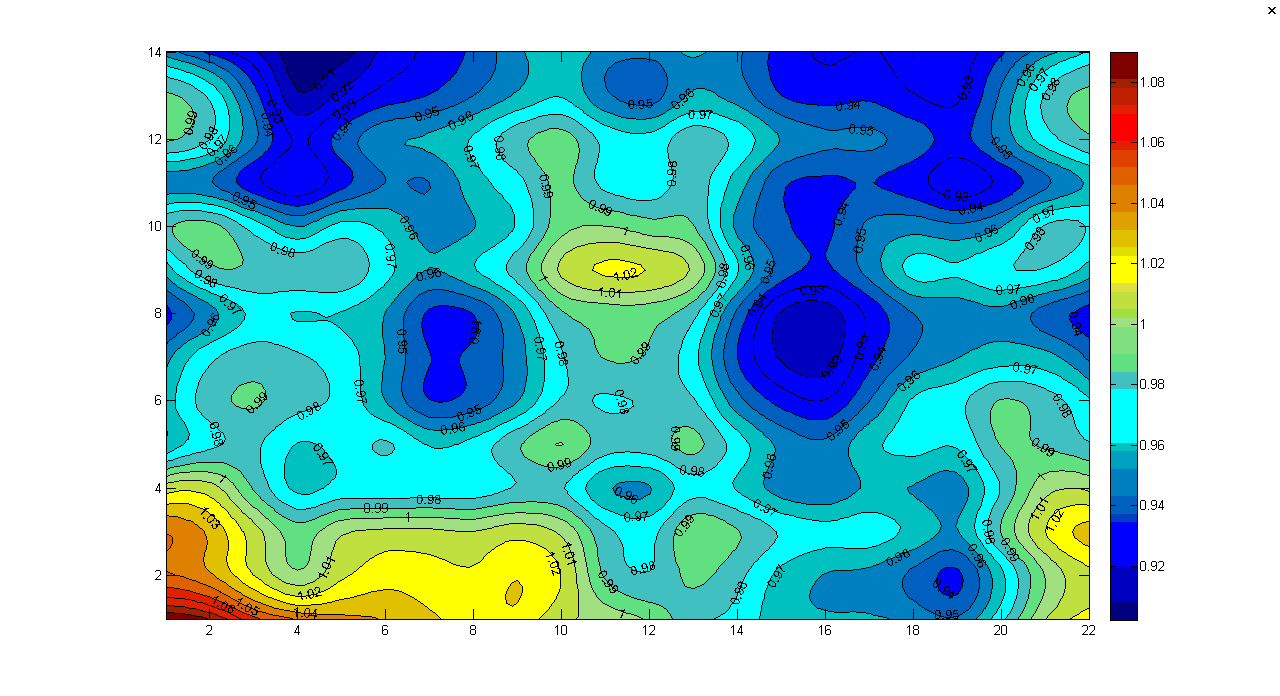
\includegraphics[width=150mm]{img/karte1.png}
\caption[Relative Verteilung der Einstrahlung]{Relative Verteilung der Einstrahlung}\label{karte1}
\end{figure}

\begin{figure}[htbp]
\centering
\includegraphics[width=150mm]{img/vergleich23.png}
\caption{Vergleich zweier Messungen}\label{vergleich}
\end{figure}

\begin{figure}[htbp]
\centering
\includegraphics[width=150mm]{img/tempm1.png}
\caption[Temperatur der Zelle]{Temperatur der Zelle}\label{tm1}
\end{figure}

\begin{figure}[htbp]
\centering
\includegraphics[width=150mm]{img/tempm2.png}
\caption[konstante Temperatur der Zelle]{konstante Temperatur der Zelle}\label{tm2}
\end{figure}


\section{Vermessung der Ausleuchtung einzelner Lampen}

Die geringe Messzeit des Roboters, verglichen mit der mechanischen Methode, macht es möglich die Bestrahlungsstärkeverteilung der einzelnen Lampen in realistischer Zeit zu bestimmen.
Veränderbar sind der Abstand zwischen Lampenfeld und Prüfebene. Die Leistungen der Lampen lassen sich einzeln steuern. 
Die Lampen wurden einzeln mit einer Lampenleistung von 100\% vermessen, die anderen Lampen waren jeweils auf 0\%. Aus den Werten der Einzelmessung wurde optimierte Gesamtausleuchtung errechnet. Diese optimierte Einstellung (welche noch zu messen ist) wird den Herstellerangaben verglichen. Dann wir sich zeigen ob die Methode erfolgsversprechend ist.
Einfacher Algorimus für Matlab:
- Leistung einzelner Lampen nur zwischen 100 und 80%: 
- Eine der mittleren Lampen auf 100\% festsetzen, andere Lampen in einem Bereich von 80\% bis 100\% varieren lassen. Nicht alle Lampen alle 20 Schritte machen lassen. 20 hoch 9 wären sehr viele Rechenschritte.

Zuerst muss eine Lampe bei verschiedenen Einstellungen (100, 90, 80 \%) gemessen werden, um den Zusammenhang von Einstellung der Lampenleistung mit der gemessenen Bestrahlungsstärke zu ermitteln.

\begin{figure}
    \subfigure[3D Ansicht]{\includegraphics[width=0.49\textwidth]{img/E1.png}}
    \subfigure[Landkarte]{\includegraphics[width=0.49\textwidth]{img/E1a.png}}
\caption{Lampe E1}
\end{figure} 

\begin{figure}
    \subfigure[3D Ansicht]{\includegraphics[width=0.49\textwidth]{img/E2.png}}
    \subfigure[Landkarte]{\includegraphics[width=0.49\textwidth]{img/E2a.png}}
\caption{Lampe E2}
\end{figure} 

\begin{figure}
    \subfigure[3D Ansicht]{\includegraphics[width=0.49\textwidth]{img/E3.png}}
    \subfigure[Landkarte]{\includegraphics[width=0.49\textwidth]{img/E3a.png}}
\caption{Lampe E3}
\end{figure}

\begin{figure}
    \subfigure[3D Ansicht]{\includegraphics[width=0.49\textwidth]{img/E4.png}}
    \subfigure[Landkarte]{\includegraphics[width=0.49\textwidth]{img/E4a.png}}
\caption{Lampe E4}
\end{figure} 

\begin{figure}
    \subfigure[3D Ansicht]{\includegraphics[width=0.49\textwidth]{img/E5.png}}
    \subfigure[Landkarte]{\includegraphics[width=0.49\textwidth]{img/E5a.png}}
\caption{Lampe E5}
\end{figure} 

\begin{figure}
    \subfigure[3D Ansicht]{\includegraphics[width=0.49\textwidth]{img/E6.png}}
    \subfigure[Landkarte]{\includegraphics[width=0.49\textwidth]{img/E6a.png}}
\caption{Lampe E6}
\end{figure} 

\begin{figure}
    \subfigure[3D Ansicht]{\includegraphics[width=0.49\textwidth]{img/E7.png}}
    \subfigure[Landkarte]{\includegraphics[width=0.49\textwidth]{img/E7a.png}}
\caption{Lampe E7}
\end{figure} 

\begin{figure}
    \subfigure[3D Ansicht]{\includegraphics[width=0.49\textwidth]{img/E8.png}}
    \subfigure[Landkarte]{\includegraphics[width=0.49\textwidth]{img/E8a.png}}
\caption{Lampe E8}
\end{figure} 

\begin{figure}
    \subfigure[3D Ansicht]{\includegraphics[width=0.49\textwidth]{img/E9.png}}
    \subfigure[Landkarte]{\includegraphics[width=0.49\textwidth]{img/E9a.png}}
\caption{Lampe E9}
\end{figure} 

\begin{figure}
    \subfigure[3D Ansicht]{\includegraphics[width=0.49\textwidth]{img/E10.png}}
    \subfigure[Landkarte]{\includegraphics[width=0.49\textwidth]{img/E10a.png}}
\caption{Lampe E10}
\end{figure} 





 





\section{Schlussfolgerung}\thispagestyle{empty}

Der Roboter erleichtert die Messung der Bestrahlungsstärkemessung enorm. Durch die kurze Messdauer ist es möglich die Bestrahlungsstärke in periodischen Zeitabständen zu vermessen, um so die Alterung der Lampen zu dokumentieren. 
Diese Art von Messroboter kann in jedem stationären Sonnensimulator entsprechender Größe zur Vermessung der Bestrahlungsstärkeverteilung verwendet werden. 
Die Verwendung des Messroboters erlaubt die Bestrahlungsstärkeverteilung einzelner Lampen zu ermitteln.
Ebenso die Bestrahlungsstärkeverteilung bei unterschiedlichen Höhen des Lampenfeldes.
Die 3D-Drucktechnik versprach zwar eine schnelle Entwicklung, sprich ein Rapid Prototyping, insgesamt benötigen die gedruckten Räder eine aufwendige Nachbearbeitung, damit sie überhaupt zusammengebaut werden konnten. Und auch im Laufe des Roboterlebens sind alle mechanischen Probleme bei den Rädern aufgetretten. Sei es dass sich die Räder von selbst gelockert haben. Sei dass sich Kugellager aus der Verklebung gelöst haben. 


% Literaturverzeichnis
% Das Literaturverzeichnis kann auch nach einem allf"alligen Anhang positiioniert werden (siehe "`Leitfaden f"ur Bachelor- und Diplomarbeiten"', Version 2.0, Abschnitt 2.9).

% M"oglichkeit 1: Erzeugung des Literaturverzeichnisses mit BibTeX:
% Die Quellen sind in der Datei *.bib (hier Literatur.bib) einzugeben. Danach muss diese Vorlage einmal geTeXt werden, dann BibTeX angewendet werden und 
% anschliessend nochmals zweimal geTeXt werden.
% Im Text erfolgt die Zitierung mit dem Anker-Schl"usselwort, z.B. \cite{kop05}.
\bibliographystyle{IEEEtran}
\bibliography{Literatur}

% M"oglichkeit 2: Erzeugung eines Literaturverzeichnisses ohne BibTeX:
%\begin{thebibliography}{99}
%\bibitem[kop05]{kop05}
%H.~Kopka, {\em LaTeX, Band 1: Einf"uhrung}, Pearson Studium, M"unchen, 3.~Auflage, 2005.
%\bibitem[knu98]{knu98}
%F.~Mittelbach, M.~Goossens, J.~Braams, D.~Carlisle, and Ch. Rowley, {\em The LaTeX Companion}, 
%Addison-Wesley, 2nd edition, 2004.
%\end{thebibliography}

% Abbildungsverzeichnis
\listoffigures
\addcontentsline{toc}{chapter}{Abbildungsverzeichnis} % f"ugt den Eintrag "Abbildungsverzeichnis" im Inhaltsverzeichnis hinzu
\newpage

% Tabellenverzeichnis
\listoftables 
\addcontentsline{toc}{chapter}{Tabellenverzeichnis} % f"ugt den Eintrag "Tabellenverzeichnis" im Inhaltsverzeichnis hinzu
\newpage

% Abk"urzungsverzeichnis
% Bei Verwendung der Dokumentklasse "scrartcl" ist der Befehlt \addchap{Abk"urzungsverzeichnis} durch 
% \addsec{Abk"urzungsverzeichnis} zu ersetzen
\addchap{Abk"urzungsverzeichnis}
\hspace{-17mm}\begin{tabular}{>{\raggedleft}p{0.2\linewidth} p{0.75\linewidth} p{0.1\linewidth}}
www & World Wide Web \\
URL & Uniform Resource Locator
\end{tabular}


% Anh"ange
\begin{appendix}
\chapter{Sourcecode Arduino}

\begin{verbatim}
/*
Programm zum Steuern des Sonnensimulatormessroboters
Version 1.1 
*/

#include <SD.h>

void vor(int sped);
void zuruck(int sped);
void left(int sped);
void right(int sped);
void tl(int sped);
void tr(int sped);
void ztl();
void ztr();
void vtl();
void vtr();
void halt(); 

// ADCs zum Auslesen der 3x3 Matrix
const int analogInPin0 = A9;  
const int analogInPin1 = A2;
const int analogInPin2 = A5;
const int analogInPin3 = A8;
const int analogInPin4 = A1;
const int analogInPin5 = A4;
const int analogInPin6 = A7;
const int analogInPin7 = A0;
const int analogInPin8 = A3;
const int analogInPin9 = A6;

// Ausgang zum Schalten der Infrarot-Leds
const int analogInPin10 = A10;

// button pin
int button = 21; 

// ADC für Messwerte
const int analogInPin12 = A12;
const int analogInPin13 = A13;
const int analogInPin14 = A14;
const int analogInPin15 = A15;

// Digitalausgänge zum Ansteuern der Motoren
int IN1M1 = 2;
int IN2M1 = 3;
int IN1M2 = 4;
int IN2M2 = 5;
int IN1M3 = 6;
int IN2M3 = 9;
int IN1M4 = 7;
int IN2M4 = 8;

// Sensorwerte der optischen Sensoren (beleuchtet)
int sensorValue0 = 0;        // value read from the pot
int sensorValue1 = 0;        // value read from the pot
int sensorValue2 = 0;        // value read from the pot
int sensorValue3 = 0;        // value read from the pot
int sensorValue4 = 0;        // value read from the pot
int sensorValue5 = 0;        // value read from the pot
int sensorValue6 = 0;        // value read from the pot
int sensorValue7 = 0;        // value read from the pot
int sensorValue8 = 0;        // value read from the pot
int sensorValue9 = 0;        // value read from the pot

// Sensorwerte der optischen Sensoren (unbeleuchtet)
int sensorValue0d = 0;        // value read from the pot
int sensorValue1d = 0;        // value read from the pot
int sensorValue2d = 0;        // value read from the pot
int sensorValue3d = 0;        // value read from the pot
int sensorValue4d = 0;        // value read from the pot
int sensorValue5d = 0;        // value read from the pot
int sensorValue6d = 0;        // value read from the pot
int sensorValue7d = 0;        // value read from the pot
int sensorValue8d = 0;        // value read from the pot
int sensorValue9d = 0;        // value read from the pot

// für Auswertung der opischen Sensoren
int A = 0;
int B = 0;
int C = 0;
int D = 0;
int E = 0;
int F = 0;
int G = 0;
int H = 0;
int I = 0;
int S = 0;

// Grenzwerte für hell (=white) und dunkel (=bleak)
int white = 400;
int white2 = 250;
int bleak = 100;
int bleak2 = 150;

// zur Berechnung der Lage der LInie
float x1,x2,x3,d,k;
float y1,y2,y3,d2,k2;

// einige Hilfsvariablen
char mode='s';
char richtung='v';
int _stop=0;
int vor_ein=0;
int zuruck_ein=0;

// für die Auswertung der Messwerte
long int  temp_modul = 0; 
long int temp_i=0;
long int _Isc = 0; 
long int time = 0; 

// zur Schreiben auf die SD Karte
const int chipSelect = 53;

// Zählvariable für Messpunkt, Spalte und Reihe
int count = 0;
int count2 = 0;
int row = 1;

// zur Schreiben auf die SD Karte
String dataString = "";

// notwendig für die Kommunikation mit SD Karte
void setup() {
  pinMode(A10, OUTPUT);
  pinMode(53, OUTPUT);
  Serial.begin(9600); 
  analogReference(EXTERNAL);
  SD.begin(chipSelect);
  pinMode(button, INPUT);
}

// Definiert alle möglichen Bewegungen
void zuruck(int sped)  //speed ist besetzt!
{
  analogWrite(IN1M1,0);
  analogWrite(IN2M1,sped);   
  analogWrite(IN1M2,0);
  analogWrite(IN2M2,sped); 
  analogWrite(IN1M3,0);
  analogWrite(IN2M3,sped); 
  analogWrite(IN1M4,0);
  analogWrite(IN2M4,sped);
}  

void vor(int sped)  //speed ist besetzt!
{
  analogWrite(IN1M1,sped);
  analogWrite(IN2M1,0);   
  analogWrite(IN1M2,sped);
  analogWrite(IN2M2,0); 
  analogWrite(IN1M3,sped);
  analogWrite(IN2M3,0); 
  analogWrite(IN1M4,sped);
  analogWrite(IN2M4,0);
}

void left(int sped)  //speed ist besetzt!
{
  analogWrite(IN1M1,0);
  analogWrite(IN2M1,sped);   
  analogWrite(IN1M2,sped);
  analogWrite(IN2M2,0); 
  analogWrite(IN1M3,sped);
  analogWrite(IN2M3,0); 
  analogWrite(IN1M4,0);
  analogWrite(IN2M4,sped);
}

void right(int sped)  //speed ist besetzt!
{
  analogWrite(IN1M1,sped);
  analogWrite(IN2M1,0);   
  analogWrite(IN1M2,0);
  analogWrite(IN2M2,sped); 
  analogWrite(IN1M3,0);
  analogWrite(IN2M3,sped); 
  analogWrite(IN1M4,sped);
  analogWrite(IN2M4,0);
}

void tr(int sped)
{
  analogWrite(IN1M1,sped);
  analogWrite(IN2M1,0);   
  analogWrite(IN1M2,0);
  analogWrite(IN2M2,sped); 
  analogWrite(IN1M3,sped);
  analogWrite(IN2M3,0); 
  analogWrite(IN1M4,0);
  analogWrite(IN2M4,sped);
}

void tl(int sped)
{
  analogWrite(IN1M1,0);
  analogWrite(IN2M1,sped);   
  analogWrite(IN1M2,sped);
  analogWrite(IN2M2,0); 
  analogWrite(IN1M3,0);
  analogWrite(IN2M3,sped); 
  analogWrite(IN1M4,sped);
  analogWrite(IN2M4,0);
}

void vtr()
{   
  analogWrite(IN1M1,64);
  analogWrite(IN2M1,0);   
  analogWrite(IN1M2,0);
  analogWrite(IN2M2,64); 
  analogWrite(IN1M3,128);
  analogWrite(IN2M3,0); 
  analogWrite(IN1M4,128);
  analogWrite(IN2M4,0);
}

void vtl()
{   
  analogWrite(IN1M1,0);
  analogWrite(IN2M1,64);   
  analogWrite(IN1M2,64);
  analogWrite(IN2M2,0); 
  analogWrite(IN1M3,128);
  analogWrite(IN2M3,0); 
  analogWrite(IN1M4,128);
  analogWrite(IN2M4,0);
}

void ztr()  //speed ist besetzt!
{
  analogWrite(IN1M1,0);
  analogWrite(IN2M1,64);   
  analogWrite(IN1M2,0);
  analogWrite(IN2M2,64); 
  analogWrite(IN1M3,0);
  analogWrite(IN2M3,64); 
  analogWrite(IN1M4,64);
  analogWrite(IN2M4,0);
}  

void ztl()  //speed ist besetzt!
{
  analogWrite(IN1M1,0);
  analogWrite(IN2M1,64);   
  analogWrite(IN1M2,0);
  analogWrite(IN2M2,64); 
  analogWrite(IN1M3,64);
  analogWrite(IN2M3,0); 
  analogWrite(IN1M4,0);
  analogWrite(IN2M4,64);
}  

void halt()  //speed ist besetzt!
{
  analogWrite(IN1M1,0);
  analogWrite(IN2M1,0);   
  analogWrite(IN1M2,0);
  analogWrite(IN2M2,0); 
  analogWrite(IN1M3,0);
  analogWrite(IN2M3,0); 
  analogWrite(IN1M4,0);
  analogWrite(IN2M4,0);
}


// Hauptschleife
void loop() 
{ 
  int state = digitalRead(button);
  if (state == HIGH)
  {
    halt();

    _Isc = 0;
    temp_modul = 0;
    temp_i = 0;

    for(int i = 0; i < 500 ; i++)
    {
      _Isc = _Isc + analogRead(analogInPin13);  
      temp_modul = temp_modul + analogRead(analogInPin12); 
      temp_i = temp_i + analogRead(analogInPin15);  
      //delay(20);
    }
    _Isc = int(_Isc/500.0);
    temp_modul = int(temp_modul/500.0);
    temp_i = int(temp_i/500.0);

    Serial.print("\n I_sc = ");   
    Serial.print(_Isc);
    Serial.print("\t temp_modul = ");   
    Serial.print(temp_modul);
    Serial.print("\t temp_innen = ");   
    Serial.print(temp_i);

    delay(1000); 

  }

  else
  {

    // Werte ohne Beleuchtung:
    sensorValue0d = analogRead(analogInPin0);   
    sensorValue1d = analogRead(analogInPin1);  
    sensorValue2d = analogRead(analogInPin2);  
    sensorValue3d = analogRead(analogInPin3);  
    sensorValue4d = analogRead(analogInPin4);  
    sensorValue5d = analogRead(analogInPin5);  
    sensorValue6d = analogRead(analogInPin6);  
    sensorValue7d = analogRead(analogInPin7);  
    sensorValue8d = analogRead(analogInPin8);  
    sensorValue9d = analogRead(analogInPin9);  
    digitalWrite(A10, HIGH);  // LED ein
    delay(2); 
    // Werte mit Beleuchtung:
    sensorValue0 = analogRead(analogInPin0);   
    sensorValue1 = analogRead(analogInPin1);  
    sensorValue2 = analogRead(analogInPin2);  
    sensorValue3 = analogRead(analogInPin3);  
    sensorValue4 = analogRead(analogInPin4);  
    sensorValue5 = analogRead(analogInPin5);  
    sensorValue6 = analogRead(analogInPin6);  
    sensorValue7 = analogRead(analogInPin7);  
    sensorValue8 = analogRead(analogInPin8);  
    sensorValue9 = analogRead(analogInPin9);  
    digitalWrite(A10, LOW);

    A = sensorValue1 - sensorValue1d;
    B = sensorValue2 - sensorValue2d;
    C = sensorValue3 - sensorValue3d;
    D = sensorValue4 - sensorValue4d;
    E = sensorValue5 - sensorValue5d;
    F = sensorValue6 - sensorValue6d;
    G = sensorValue7 - sensorValue7d;
    H = sensorValue8 - sensorValue8d;
    I = sensorValue9 - sensorValue9d;

    S = sensorValue0 - sensorValue0d;

    // zum Erkennen der Linie bei vor- oder zurückfahren 
    x1 = ((C-A)/float(2*A-4*B+2*C));
    x2 = ((F-D)/float(2*D-4*E+2*F));
    x3 = ((I-G)/float(2*G-4*H+2*I));

    d = (x1 + x2 + x3)/3.; // ~ Abstand von der Ideallinie
    k = (x1-x3)/2.;  // Steigung = Verdrehung

    // zum Erkennen der Linie bei links- oder rechtsfahren
    y1 = ((G-A)/float(2*A-4*D+2*G));
    y2 = ((H-B)/float(2*B-4*E+2*H));
    y3 = ((I-C)/float(2*C-4*F+2*I));

    d2 = (y1+y2+y3)/3.;
    k2 = (y3-y1)/2.;

    if( S < bleak2) _stop=0;

    halt();

    if(E>bleak2)
    {

      switch(mode)
      {
      case 's':     // Start
        { 
          halt();
          delay(60000);  // 1 Minuten warten
          mode='v';
        }
        break;

        // Messmode
      case 'e':   // Ende
        {
          halt();
        }
        break;

      case 'm':   // Messen
        { 
          count = count + 1;  // Anzahl der Haltepunkte
          count2 = count2 + 1; 
          dataString = "";
          _stop=1;
          halt();

          delay(250);   // damit die Ströme der Fahrmotoren keinen Einfluss auf die AD-Wandlung haben

          _Isc = 0;
          temp_modul = 0;
          temp_i = 0;

          // Mittelung über jeweils 500 Messwerte
          for(int i = 0; i < 500 ; i++)
          {
            _Isc = _Isc + analogRead(analogInPin13);  
            temp_modul = temp_modul + analogRead(analogInPin12); 
            temp_i =  temp_i + analogRead(analogInPin15); 
          }
          _Isc = int(_Isc/500.0);
          temp_modul = int(temp_modul/500.0);
          temp_i = int(temp_i/500.0);
          time = millis();

          // Schreiben aud SD-Karte
          dataString += String(time);
          dataString += "\t"; 
          dataString += String(_Isc); 
          dataString += "\t"; 
          dataString += String(temp_modul); 
          dataString += "\t"; 
          dataString += String(temp_i); 
          dataString += "\t"; 
          dataString += String(count); 
          dataString += "\t"; 
          dataString += String(count2); 
          dataString += "\t"; 
          dataString += String(row); 

          // Schreibe aud SD Card
          File dataFile = SD.open("datalog.txt", FILE_WRITE);
          if (dataFile) {
            dataFile.println(dataString);
            dataFile.close();
          }

          // zurück in den Bewegungsmode
          if(richtung=='v') mode='v';
          if(richtung=='z') mode='z';

        }
        break;

      case 'v':   // Vorwärtsfahren
        { 

          richtung='v';

          if(d>0.02)  vtr();
          else 
          {  
            if(d>-0.02)  vor(128);
            else 
              vtl();
          }

          //if((C<bleak)&&(A<bleak))
          if(A<bleak2)
          {
            if(k>0.01) tr(64);
            else
            {
              if(k<-0.01) tl(64);
            }

            if(d>0.025) right(64);
            else
            {
              if(d<-0.025) left(64);
            }
          }   
          if((A>white)&&(B>white)) mode='a'; 

          if((_stop==0)&&(S>white2)) mode='m';   


        }
        break;

      case 'z': // Rückwärtsfahren
        { 

          richtung='z';

          if(d>0.02)  ztr();
          else 
          {  
            if(d>-0.02)  zuruck(128);
            else  ztl();
          }

          //if((G<bleak)&&(I<bleak))
          if(G<bleak2)
          {
            if(k>0.01) tr(64);
            else
            {
              if(k<-0.01) tl(64);
            }

            if(d>0.025) right(64);
            else
            {
              if(d<-0.025) left(64);
            }
          }
          if((G>white)&&(H>white)) mode='c';

          if((_stop==0)&&(S>white2)) mode='m';  

          if((I<bleak)&&(H<bleak)&&(G<bleak)) mode='e';

        }
        break; 

      case 'r':     //nach rechts
        {
          richtung='r';
          count2 = 0;

          right(128);
          if(D>white2)
          {
            if(d2>0.04) vor_ein=1;
            if(d2<0.02) vor_ein=0;
            if(d2<-0.04) zuruck_ein=1;
            if(d2>-0.02) zuruck_ein=0;

            if(vor_ein==1) vor(64);
            if(zuruck_ein==1) zuruck(64);

            if((vor_ein==0)&&(zuruck_ein==0))
            {
              if(k2>0.02) tr(64);
              else
              {
                if(k2<-0.02) tl(64);
              }
            }
          }

          if((D<bleak)&&(G<bleak)&&(A<bleak)) 
          { 
            mode='b';
          }

        } 
        break;

      case 'l':    // auch nach rechts 
        {
          richtung=='l';
          count2 = 0;

          right(128);
          //if((C<bleak)&&(I<bleak))
          if(D>white2)
          {
            if(d2>0.04) vor_ein=1;
            if(d2<0.02) vor_ein=0;
            if(d2<-0.04) zuruck_ein=1;
            if(d2>-0.02) zuruck_ein=0;

            if(vor_ein==1) vor(64);
            if(zuruck_ein==1) zuruck(64);

            if((vor_ein==0)&&(zuruck_ein==0))
            {
              if(k2>0.02) tr(64);
              else
              {
                if(k2<-0.02) tl(64);
              }
            }
          }

          if((D<bleak)&&(G<bleak)&&(A<bleak))
          { 
            mode='d';
          }

        } 
        break;

      case 'a':  // Um die Ecke fahren
        {
          if((A>bleak2)&&(B>bleak2)) vor(64);
          else 
          { 
            right(64);
            delay(700);
            halt();
            row = row +1 ;

            mode='r';

          }
        } 
        break; 

      case 'b':  // Um die Ecke fahren
        {

          zuruck(64);
          delay(850);
          halt();
          delay(500);

          mode='x';

        } 
        break; 

      case 'x':
        {
          if(d>0.025) right(64);

          if(d<-0.025) left(64);

          if((d<0.1)&&(d>-0.1)) mode='y';
        }
        break;

      case 'y':
        {
          if(k>0.01) tr(32);

          if(k<-0.01) tl(32);

          if((k<0.04)&&(k>-0.04)) mode='z';
        }
        break;

      case 'c':  // Um die Ecke fahren
        {
          if((H>bleak2)&&(G>bleak2 )) zuruck(64);
          else 
          { 
            right(64);
            delay(700);
            halt();
            row = row +1 ;

            mode='l';
          }
        } 
        break; 

      case 'd':  // Um die Ecke fahren
        {

          vor(64);
          delay(850);
          halt();
          delay(500);
          mode='q';

        } 
        break; 

      case 'q':
        {
          if(d>0.025) right(64);

          if(d<-0.025) left(64);

          if((d<0.1)&&(d>-0.1))       mode='p';
        }
        break;


      case 'p':
        {
          if(k>0.01) tr(32);

          if(k<-0.01) tl(32);

          if((k<0.04)&&(k>-0.04)) mode='v'; 

        }
        break;
      } 
    }   


    else 
    {  
      if((richtung=='v')||(richtung=='z'))
      {
        if((A>bleak2)||(D>bleak2)||(G>bleak2)||(C>bleak2)||(F>bleak2)||(I>bleak2))
        {
          if((A+D+G)>(C+F+I)) right(128);
          else left(128);
        }
        else halt();
      }


      if((richtung=='r')||(richtung=='l'))
      {
        if((A>bleak2)||(B>bleak2)||(C>bleak2)||(G>bleak2)||(H>bleak2)||(I>bleak2))
        {
          if((A+B+C)>(G+H+I)) vor(64);
          else zuruck(64);
        }
        else halt();
      }
    }

    delay(5); 

  }

}

\end{verbatim}

\chapter{Sourcecode Auswertung}



\begin{verbatim}

% Graphische Auswertung der Robotermesswerte

close all;
clc;
clear all;

% Öffnen der Datei, welche eine Messfahrt mit genau 308 Messwerten
% enthalten muss
fid = fopen('mess1.txt', 'r');
a = fscanf(fid, '%g %g', [7 308])     
a = a';
fclose(fid)

j=1; k=1; l=1;

% Umwandeln der 1 dimensionalen Modultemperatur ADC-Werte in eine Matrix:
for(i=0:307)
    if(mod(i,28)>13) k = 28- mod(i,28);
    else k = mod(i,14)+1;
    end
    Tm(k,l)=a(i+1,3);
    if(mod(i+1,14)==0) l=l+1;
    end
end

% Umrechnung der ADC-Werte in Temeratur:
Rm = (Tm +4038.9)/40.107;  % ADC --> Widerstand
TTm = (Rm-100.03)/0.3879;  % Widerstand --> Temperatur

j=1; k=1; l=1;

% Umwandeln der 1 dimensionalen Innentemperatur ADC-Werte in eine Matrix:
for(i=0:307)
    if(mod(i,28)>13) k = 28- mod(i,28);
    else k = mod(i,14)+1;
    end
    Ti(k,l)=a(i+1,4);
    if(mod(i+1,14)==0) l=l+1;
    end
end

% Umrechnung der ADC-Werte in Temeratur:
Ri = (Ti +4023.6)/40.027;  % ADC --> Widerstand
TTi = (Ri-100.03)/0.3879;  % Widerstand --> Temperatur

j=1; k=1; l=1;

% Umwandeln der 1 dimensionalen Kurzschlusstrom ADC-Werte in eine Matrix:
for(i=0:307)
    if(mod(i,28)>13) k = 28- mod(i,28);
    else k = mod(i,14)+1;
    end
    I(k,l)=a(i+1,2);
    if(mod(i+1,14)==0) l=l+1;
    end
end

% Umrechnung der ADC-Werte in Ampere:

A = (I +4.5766)/119.2;   % ADC --> Ampere
G_mean=0;
for i=1:14
    for j=1:22
G(i,j) = 1000 * A(i,j) / 4.99 * ( 1 - 0.00048 * (TTm(i,j) - 25));
G_mean = G_mean + G(i,j)
    end
end

G_mean = G_mean / 308;

[XI,YI] = meshgrid(1:.125:22, 1:.125:14);

Gi = interp2(G,XI,YI,'cubic'); % Interpolation

G_max = max(max(Gi));
G_min = min(min(Gi));

w = (G_max - G_min)/(G_max + G_min) * 100  % maximale Abweichung in Protzent

display(G_mean);

% Graphische Darstellung der Bestrahlungsstärke
figure;
surf(XI,YI,Gi); % in W/m2

% Bestrahlungsstärke Landkarte mit Niveaulinien
zlevs2 = 0.0:5:1000;
figure;
[C,h] = contourf(XI,YI,Gi,zlevs2);
set(h,'ShowText','on','TextStep',get(h,'LevelStep'))
colorbar;

% Graphische Darstellung der Modultemperatur
figure;
surf(TTm); 

% Graphische Darstellung der Umgebungstemperatur
figure;
surf(TTi);  

\end{verbatim} 

\end{appendix}


\end{document}
